%
% $Id: $
%
%
% Compilar a .pdf con LaTeX (pdflatex)
% Es necesario instalar Beamer (paquete latex-beamer en Debian)
%

%
% Gráficos:
% Los gráficos pueden suministrarse en PNG, JPG, TIF, PDF, MPS
% Los EPS deben convertirse a PDF (usar epstopdf)
%

\documentclass[17pt,aspectratio=169]{beamer}
\usetheme[orchid]{Hannover}
%\usebackgroundtemplate{
\includegraphics[width=\paperwidth]{format/libresoft-bg-soft.png}}
\usepackage[spanish]{babel}
\usepackage[utf8]{inputenc}
\usepackage{graphics}
\usepackage{amssymb} % Simbolos matematicos

%\definecolor{libresoftgreen}{RGB}{162,190,43}
%\definecolor{libresoftblue}{RGB}{0,98,143}

%\setbeamercolor{titlelike}{bg=libresoftgreen}

%% Metadatos del PDF.
%% \hypersetup{
%%   pdftitle={La tecnología no es neutra},
%%   pdfauthor={Jesús M. González Barahona},
%%   pdfcreator={GSyC/LibreSoft, Universidad Rey Juan Carlos},
%%   pdfproducer=PDFLaTeX,
%%   pdfsubject={},
%% }
%%

\newcommand\YUGE{\fontsize{48}{60}\selectfont}

\AtBeginSection[]
{
  {
    \usebackgroundtemplate{\includegraphics[width=\paperwidth,height=\paperheight]{\secimage}}
    \begin{frame}<beamer>

      \begin{center}
        {\YUGE\bf\insertsection}
      \end{center}
    \end{frame}
  }
  \renewcommand{\secimage}{figs/bookpages}
}

% Pixbay
% NikolayFrolochkin
% https://pixabay.com/en/book-reading-library-literature-1261800/
% License: CC0 Creative Commons
\newcommand{\secimage}{figs/bookpages}

\begin{document}

\title{Hace más de 10 años que hacía 10 años}
%\subtitle{}
\author{Jesús M. González Barahona}
\institute{Correo: jgb@gsyc.es ~~~~ Twitter: @jgbarah2 \\
  Universidad Rey Juan Carlos \\ }

\date{esLibre 2019 \\
  Granada, 21 de junio de 2019\\
{\small \url{https://jgbarah.github.io/presentations}} \\}

\frame{
\maketitle
}
%% \begin{center}
%% 
\includegraphics[width=6cm]{format/gsyc-urjc}
%% \end{center}

%% \begin{frame}

%%   {\Large
%%     \tableofcontents
%%   }

%% \end{frame}

%%---------------------------------------------------------------
%%---------------------------------------------------------------
\section{Hace algo más de 10 años...}

%%---------------------------------------------------------------
\begin{frame}
%\frametitle{}

\begin{center}
  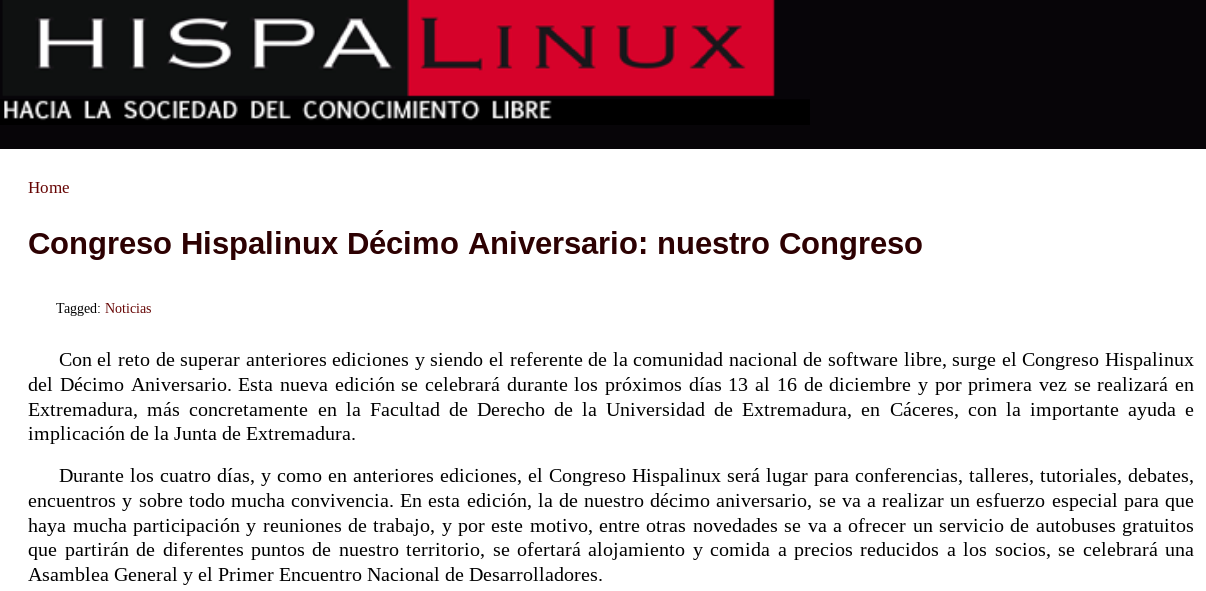
\includegraphics[width=12.5cm]{figs/hispalinux-x}
\end{center}  

\begin{flushright}
  {\small{\url{https://hispalinux.es/node/655}}}
\end{flushright}
\end{frame}

%%---------------------------------------------------------------
\begin{frame}
%\frametitle{}

\begin{center}
  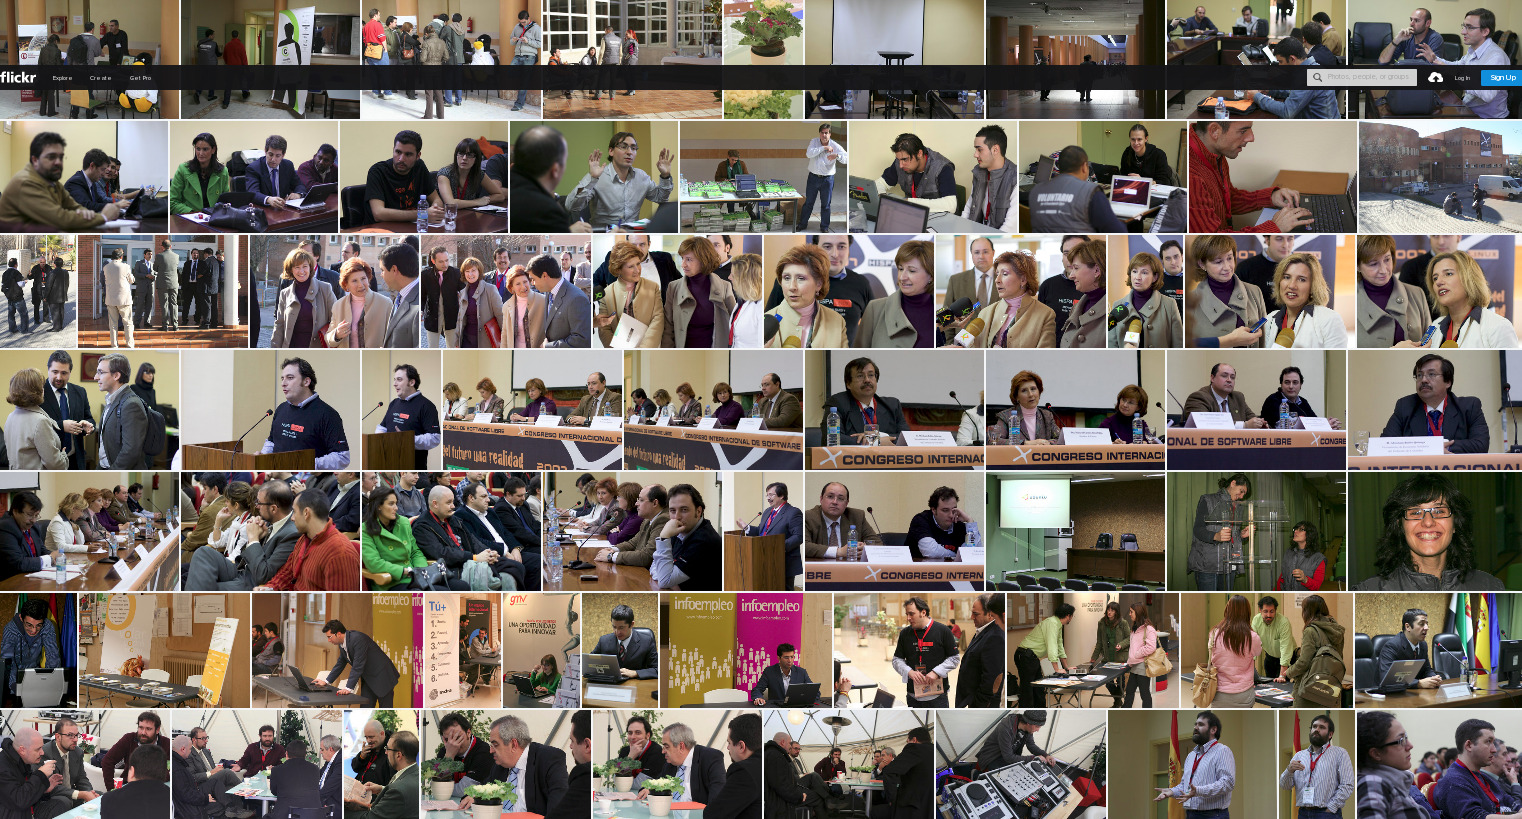
\includegraphics[width=12.5cm]{figs/hispalinux-x-fotos}
\end{center}  

\begin{flushright}
  {\scriptsize{\url{https://www.flickr.com/photos/andor/albums/72157603494343078}}}
\end{flushright}
\end{frame}

%%---------------------------------------------------------------
\begin{frame}
%\frametitle{}

\begin{center}
  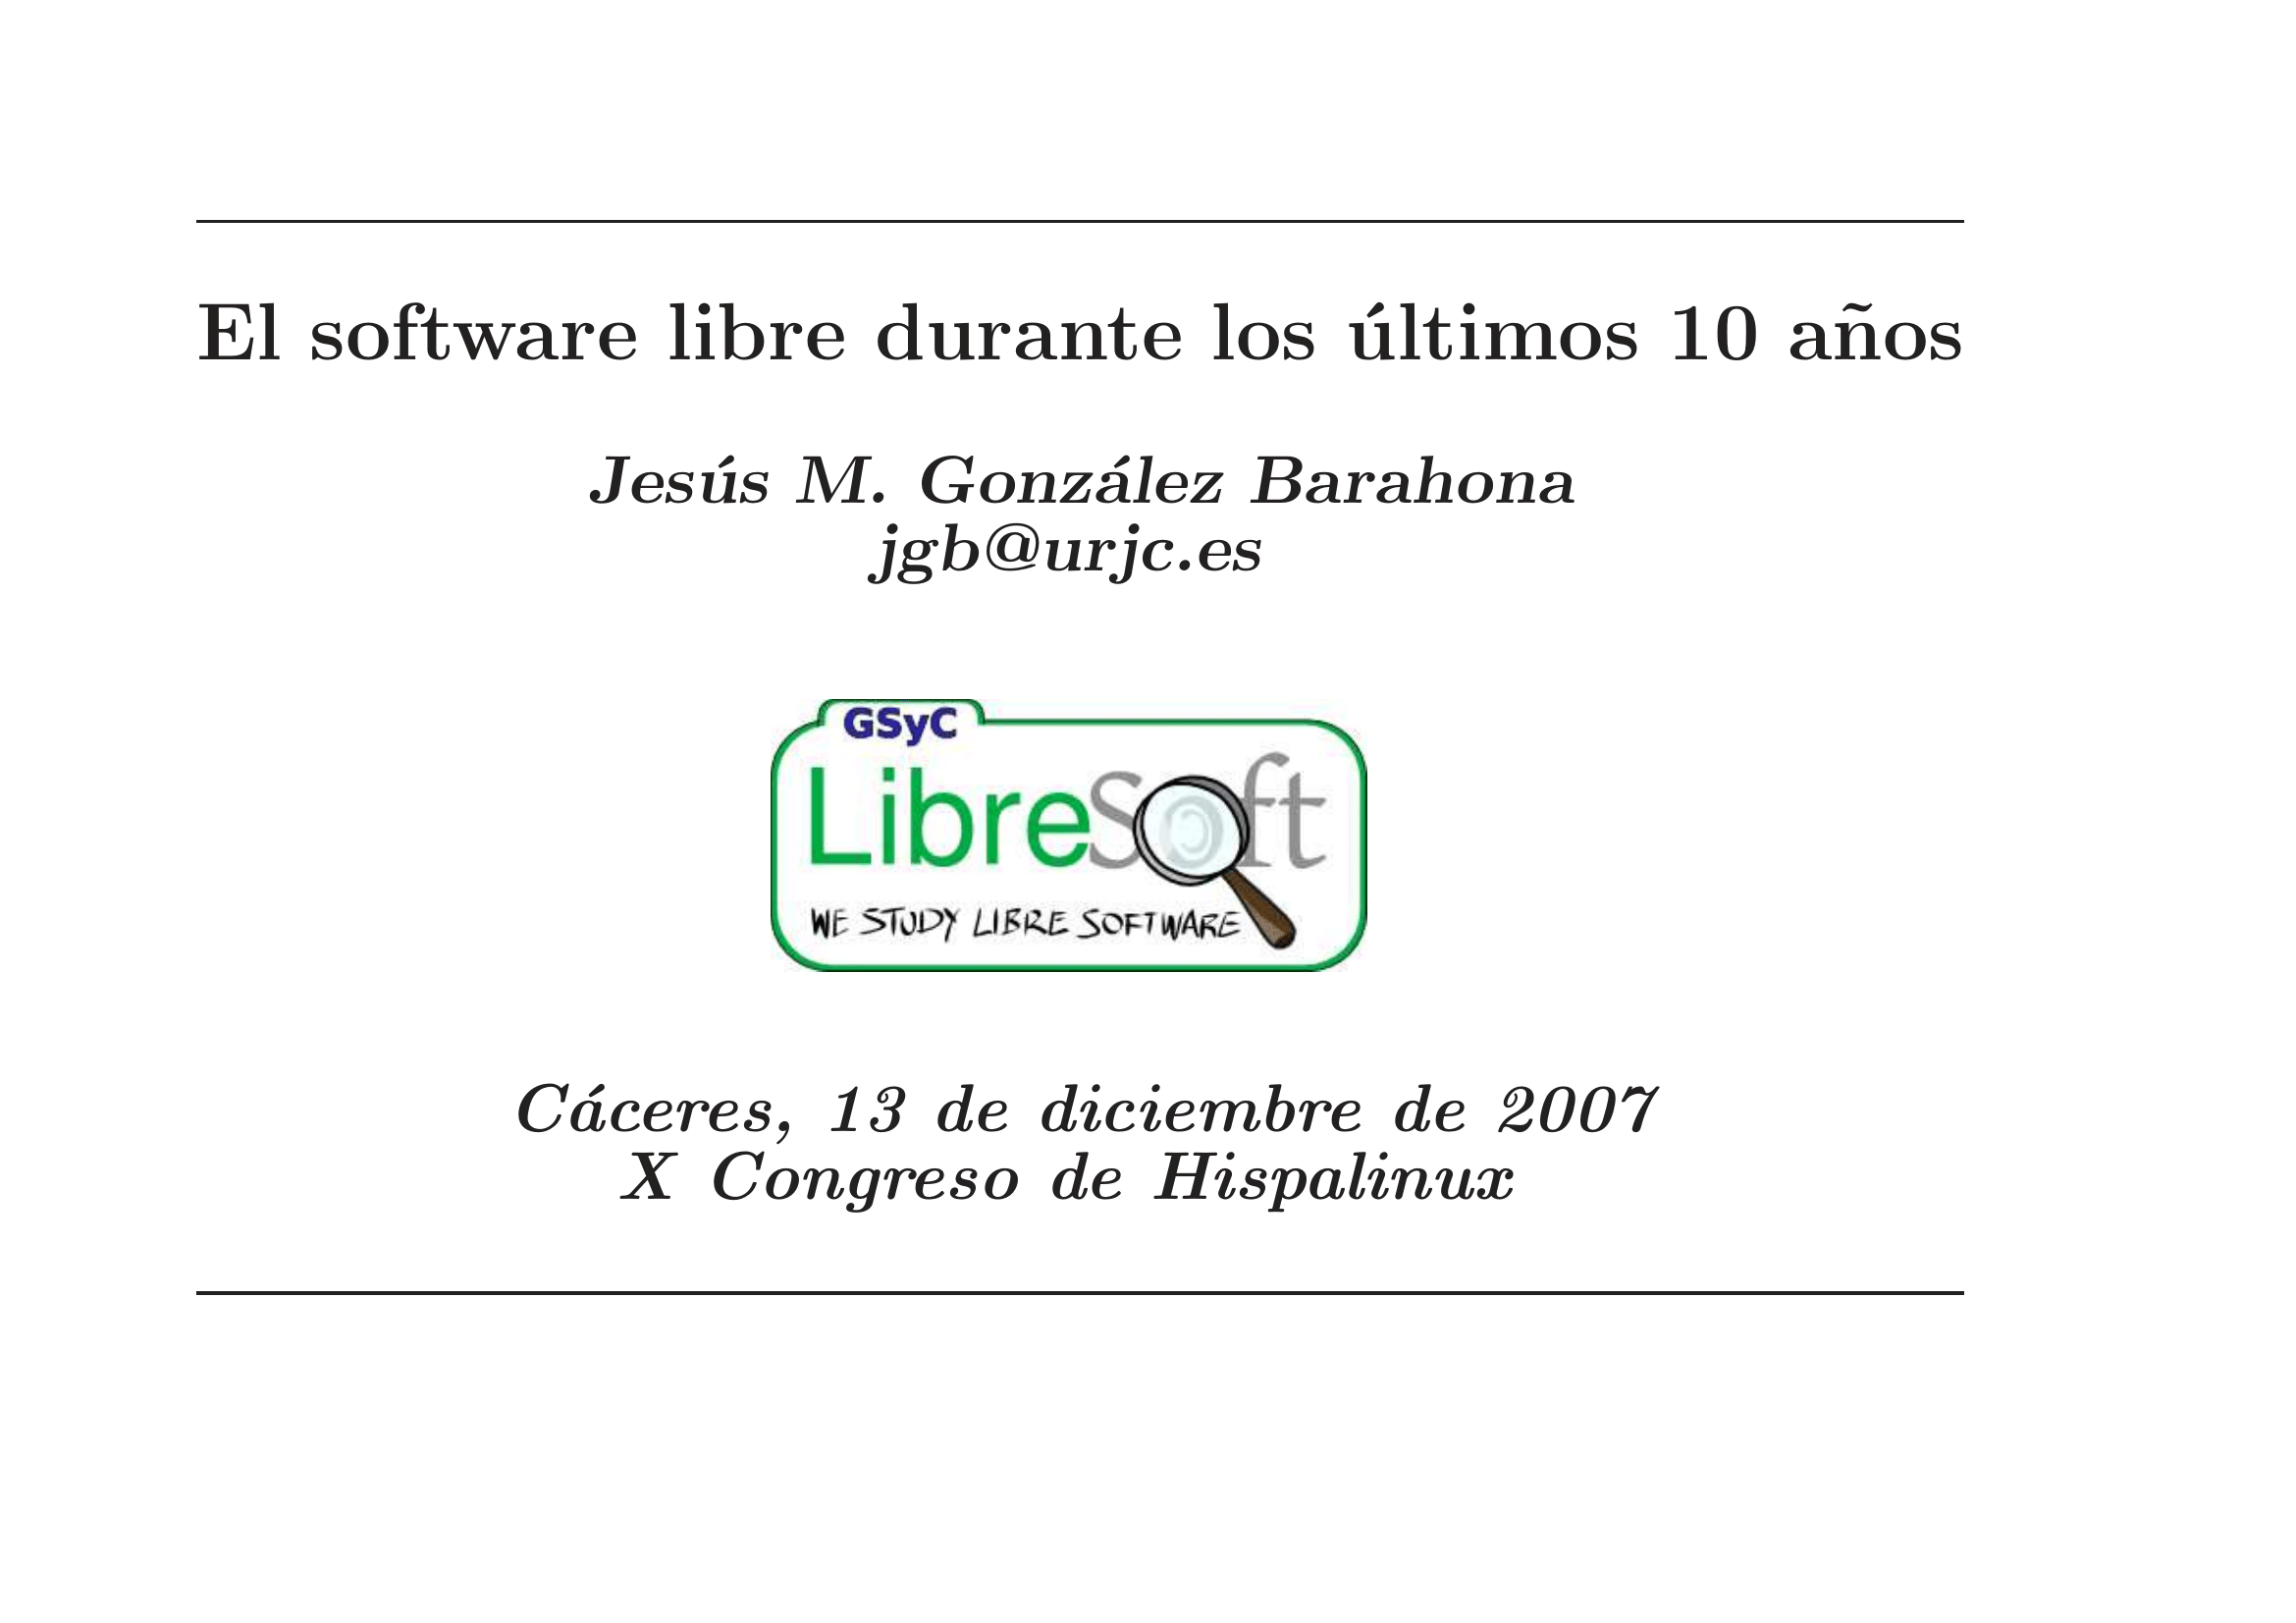
\includegraphics[width=12.5cm]{figs/transpas-01}
\end{center}

\end{frame}


%%---------------------------------------------------------------
%%---------------------------------------------------------------
\section{Recordábamos}

%%---------------------------------------------------------------
\begin{frame}
%\frametitle{}

\begin{center}
  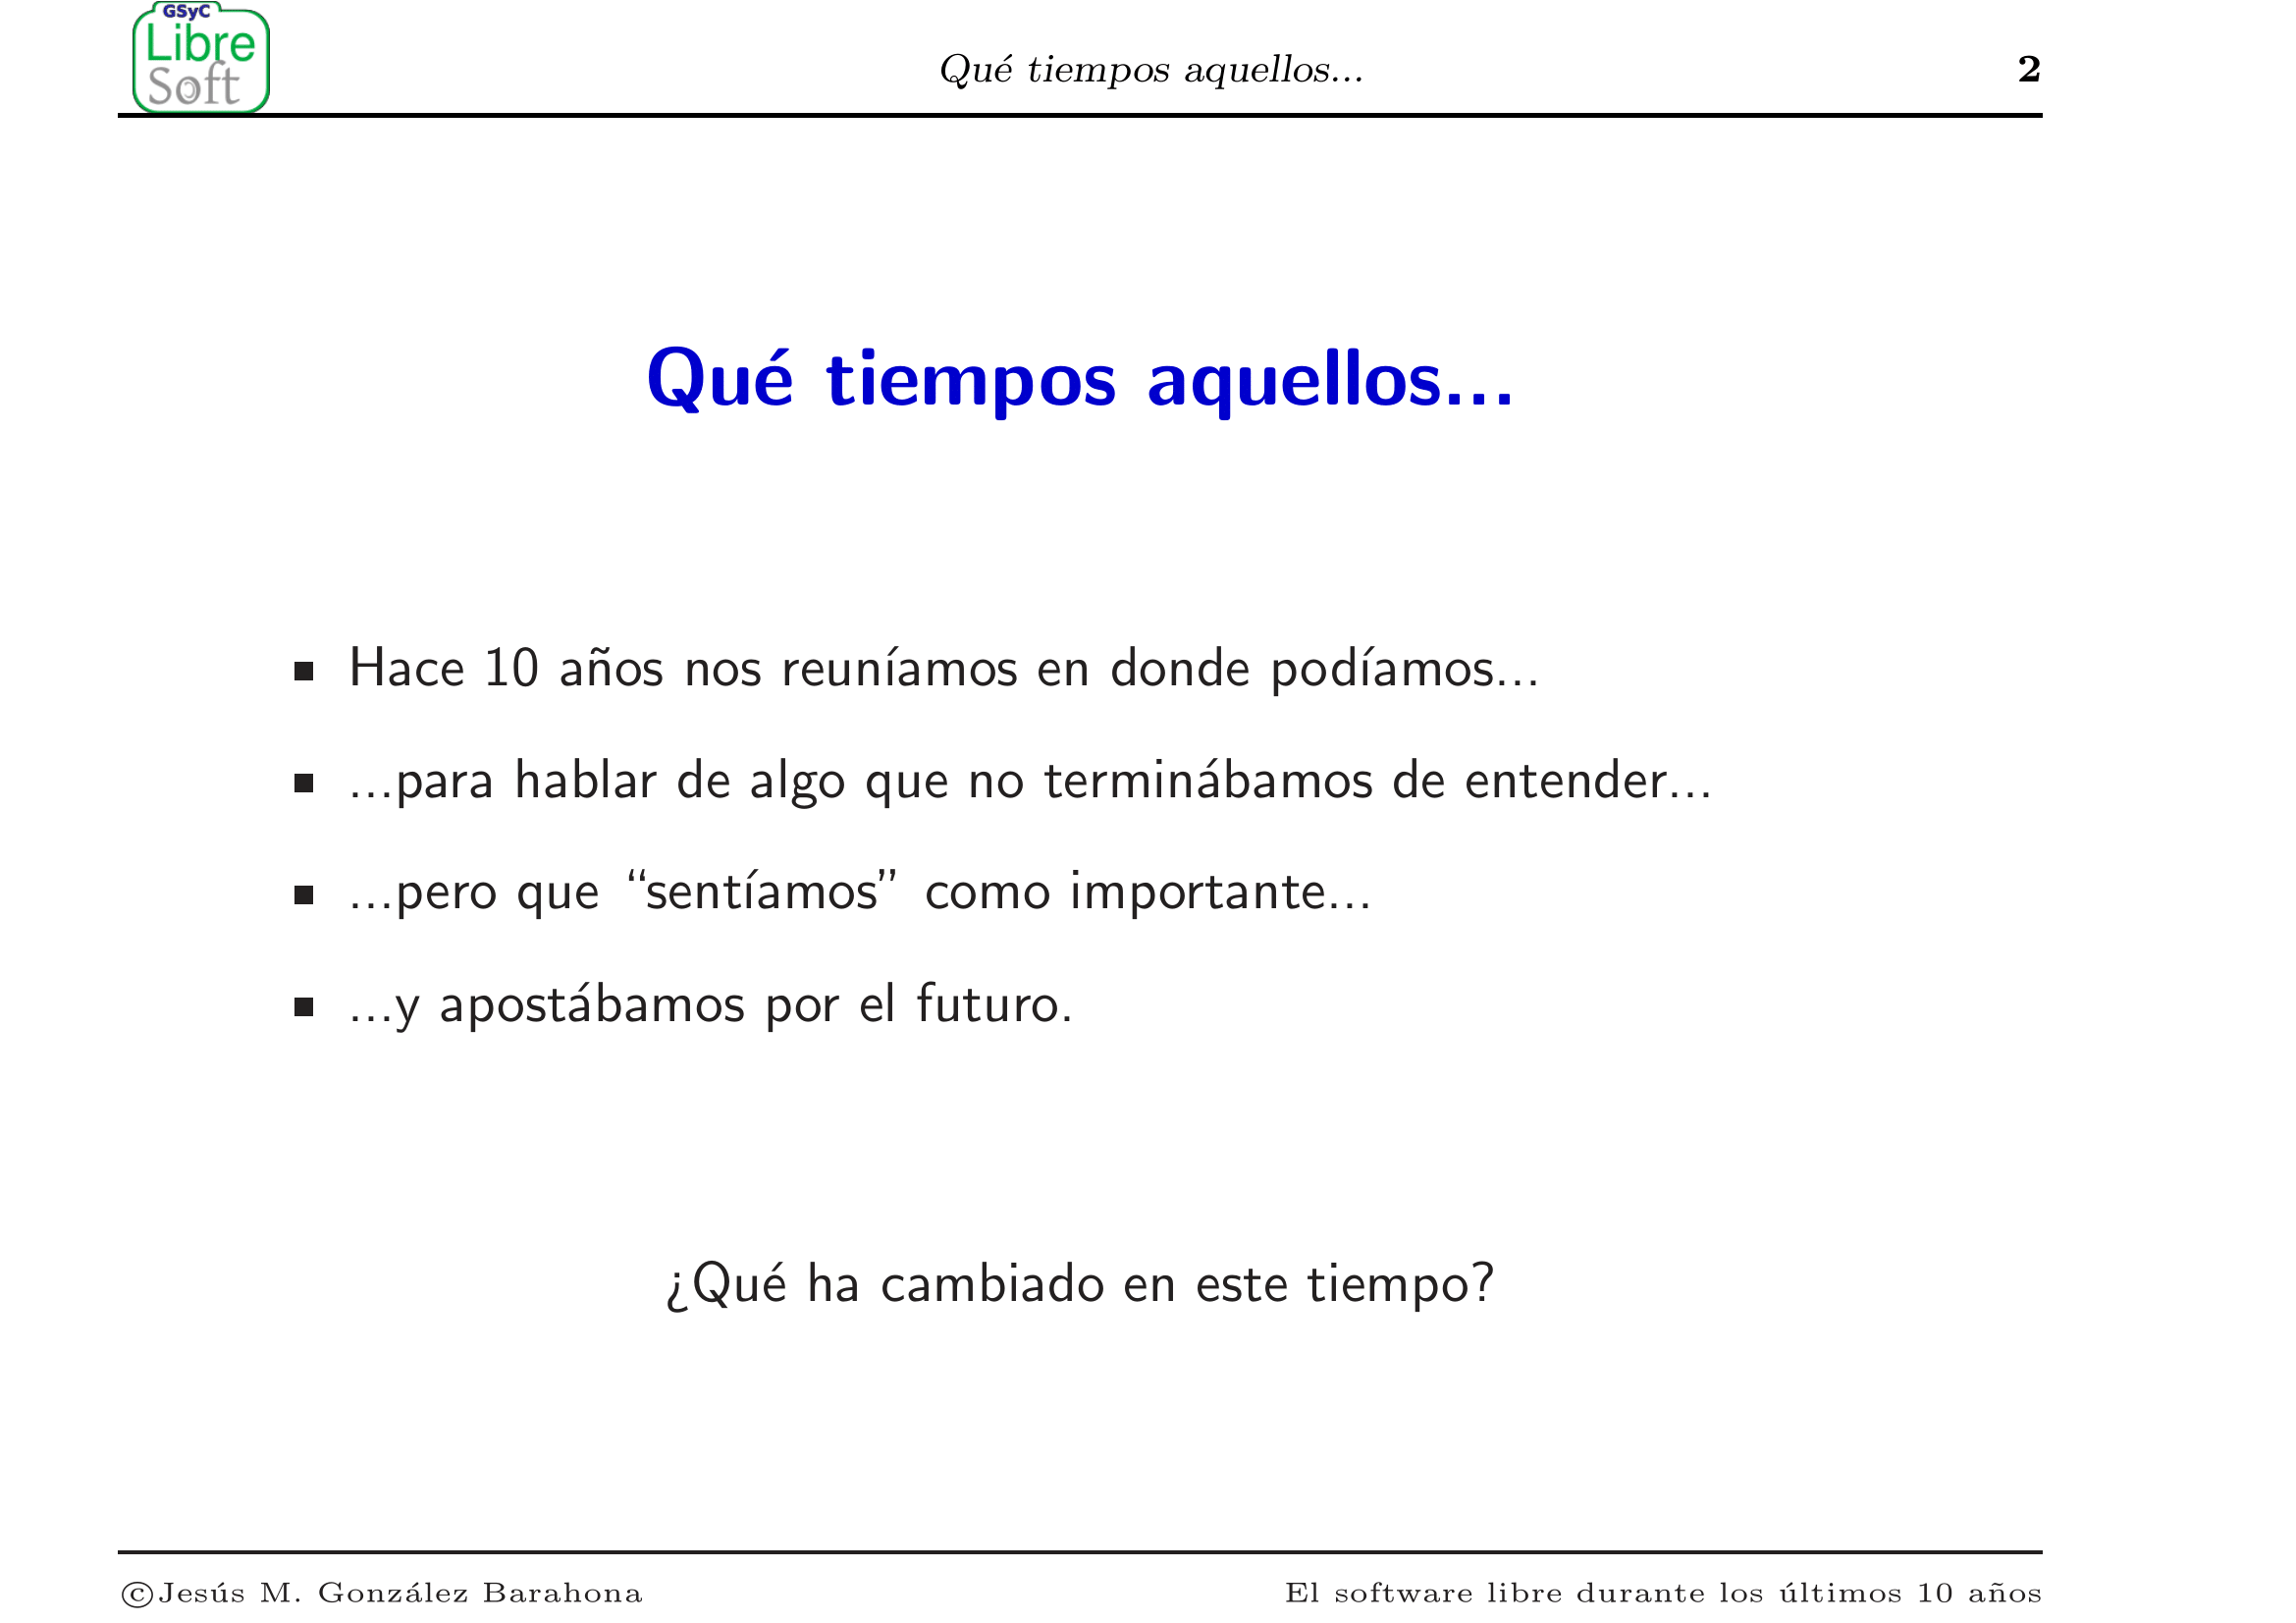
\includegraphics[width=12.5cm]{figs/transpas-03}
\end{center}  

\end{frame}

%%---------------------------------------------------------------
\begin{frame}
\frametitle{20 años después...}

\begin{itemize}
\item Entendemos algunas cosas... \\
\item pero seguimos explorando terreno sin cartografiar
\item Seguimos apostando por el futuro
\end{itemize}  

\begin{center}
  ¿Somos conscientes de lo importante que es \\
  que el software sea libre? \\
\end{center}
\end{frame}

%%---------------------------------------------------------------
\begin{frame}
\frametitle{¿Nos seguimos reuniendo?}

\begin{center}
  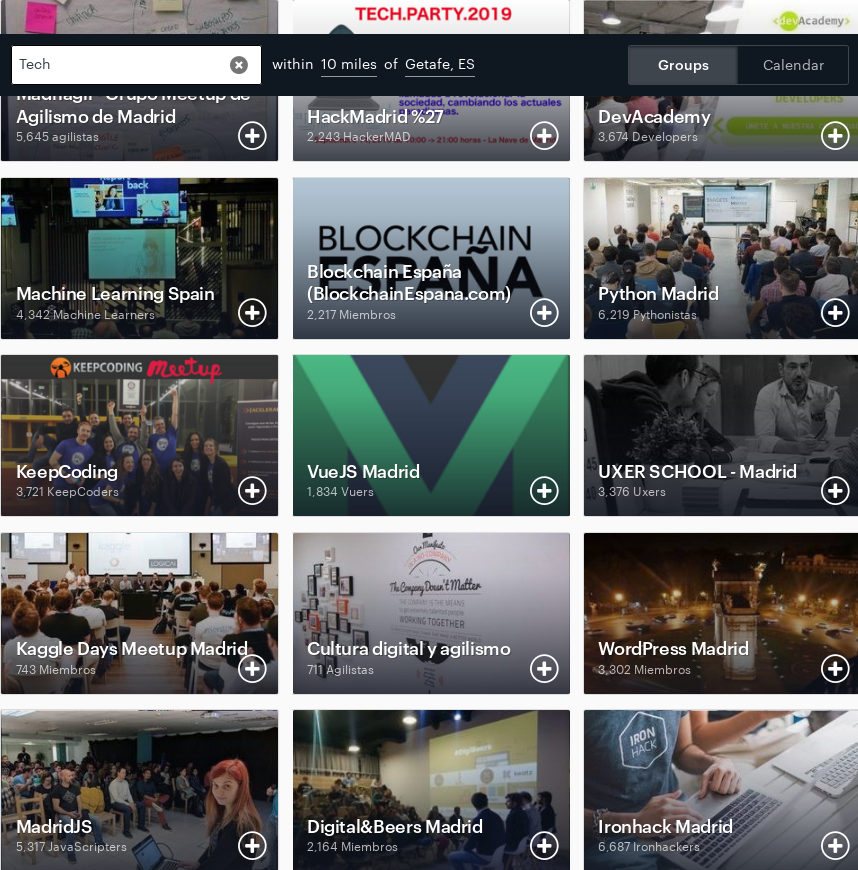
\includegraphics[width=6cm]{figs/tech-meetups-1}
  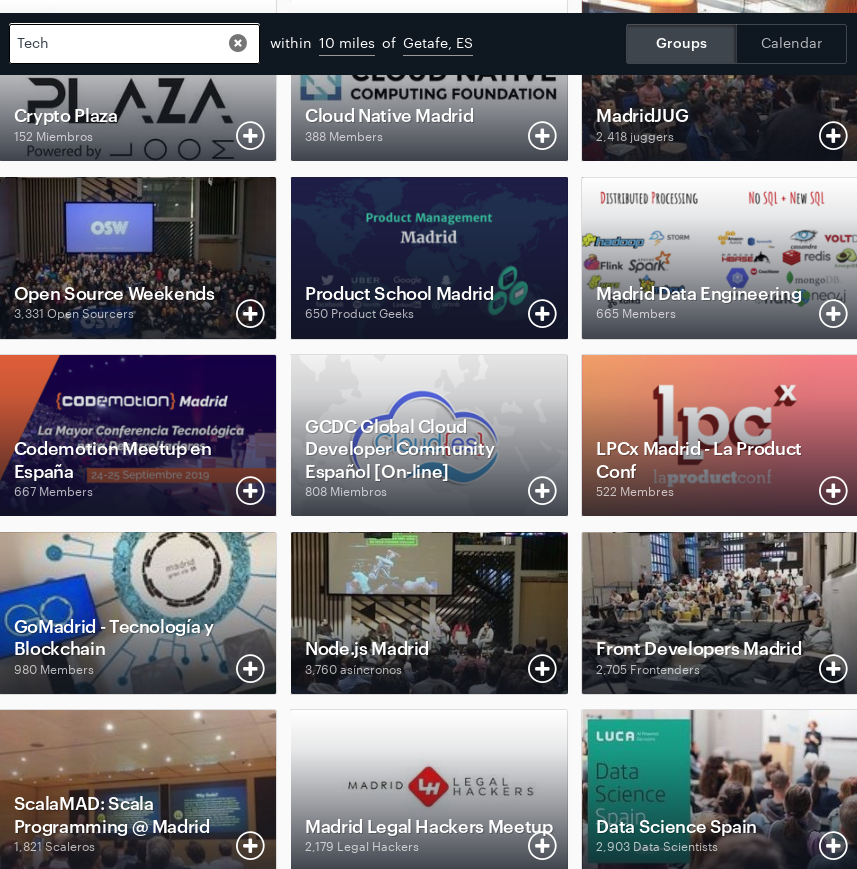
\includegraphics[width=6cm]{figs/tech-meetups-2}
\end{center}  

\end{frame}

%%---------------------------------------------------------------
\begin{frame}
\frametitle{¿Nos seguimos reuniendo?}

\begin{itemize}
\item Muchas reuniones sobre tecnologías...
\item ...libres
\end{itemize} 

\begin{center}
  ¿Ya no nos centramos en entender \\
  las implicaciones de que sean libres? \\
\end{center}

\end{frame}

%%---------------------------------------------------------------
%%---------------------------------------------------------------
\section{Creíamos que sabíamos}

%%---------------------------------------------------------------
\begin{frame}
%\frametitle{}

\begin{center}
  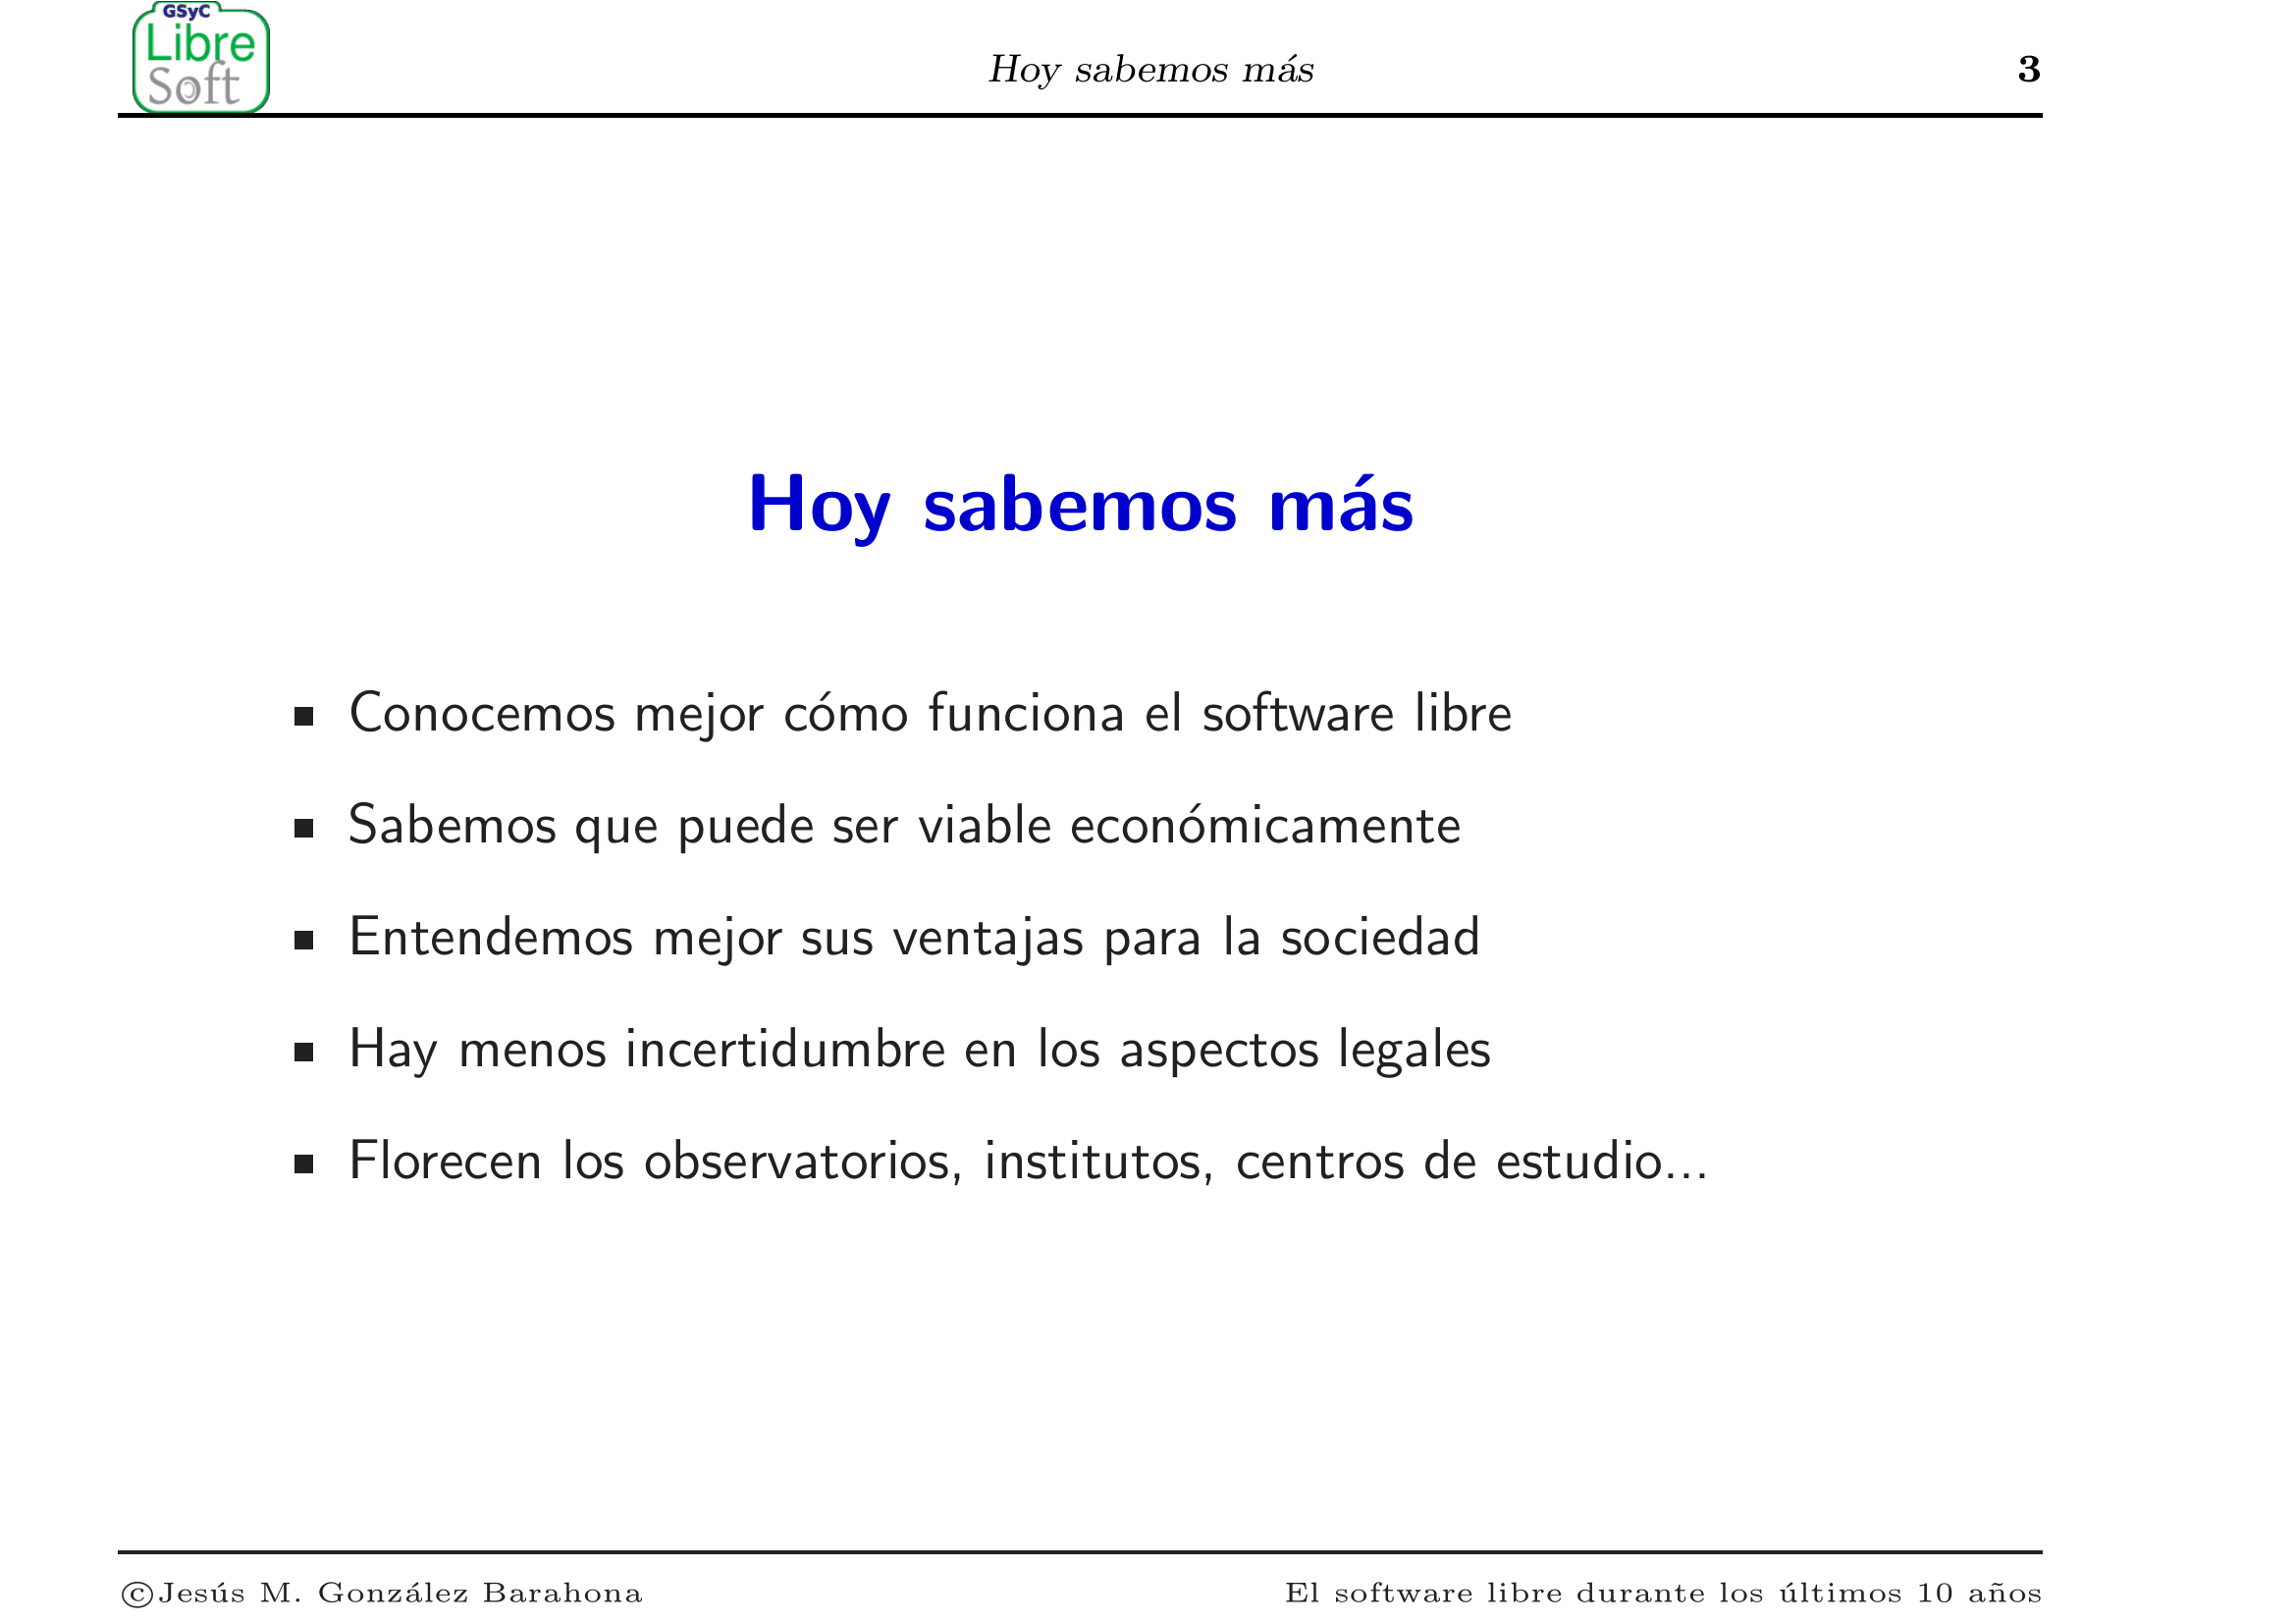
\includegraphics[width=12.5cm]{figs/transpas-04}
\end{center}  

\end{frame}

%%---------------------------------------------------------------
\begin{frame}
\frametitle{Hemos seguido aprendiendo}

\begin{itemize}
\item Mucha más experiencia
\item Las tecnologías, el modo de desarrollo \\
  se enseñan en las Universidades \\
\end{itemize} 

\begin{center}
  Pero seguimos sin saber \\
  cómo garantizar sostenibilidad \\
  incluso para proyectos críticos \\
\end{center}

\end{frame}

%%---------------------------------------------------------------
\begin{frame}

\begin{center}
  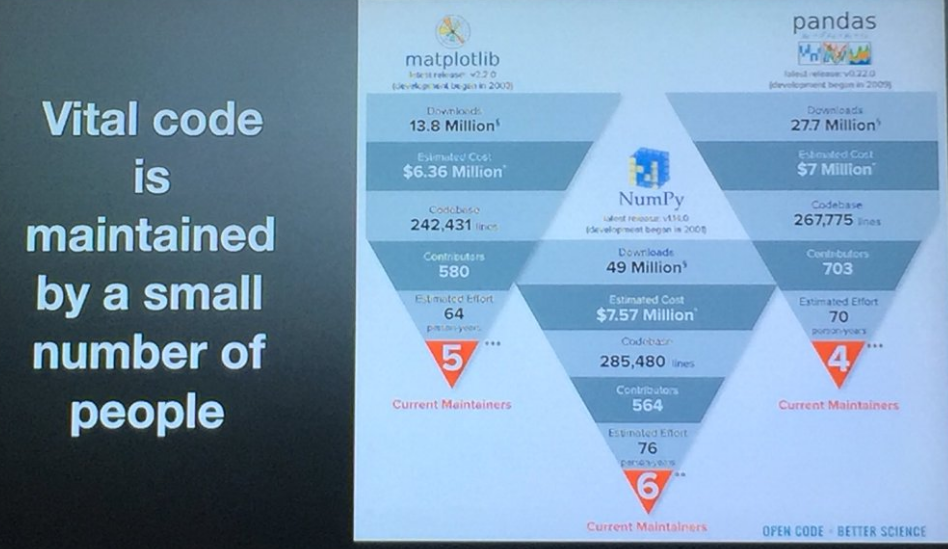
\includegraphics[width=11cm]{figs/few-maintainers}
\end{center}  

\begin{flushright}
  {\scriptsize \url{https://twitter.com/fringetracker/status/991796881767436288}}
\end{flushright}
\end{frame}

%%---------------------------------------------------------------
%%---------------------------------------------------------------
\section{Nos contábamos}

%%---------------------------------------------------------------
\begin{frame}
%\frametitle{}

\begin{center}
  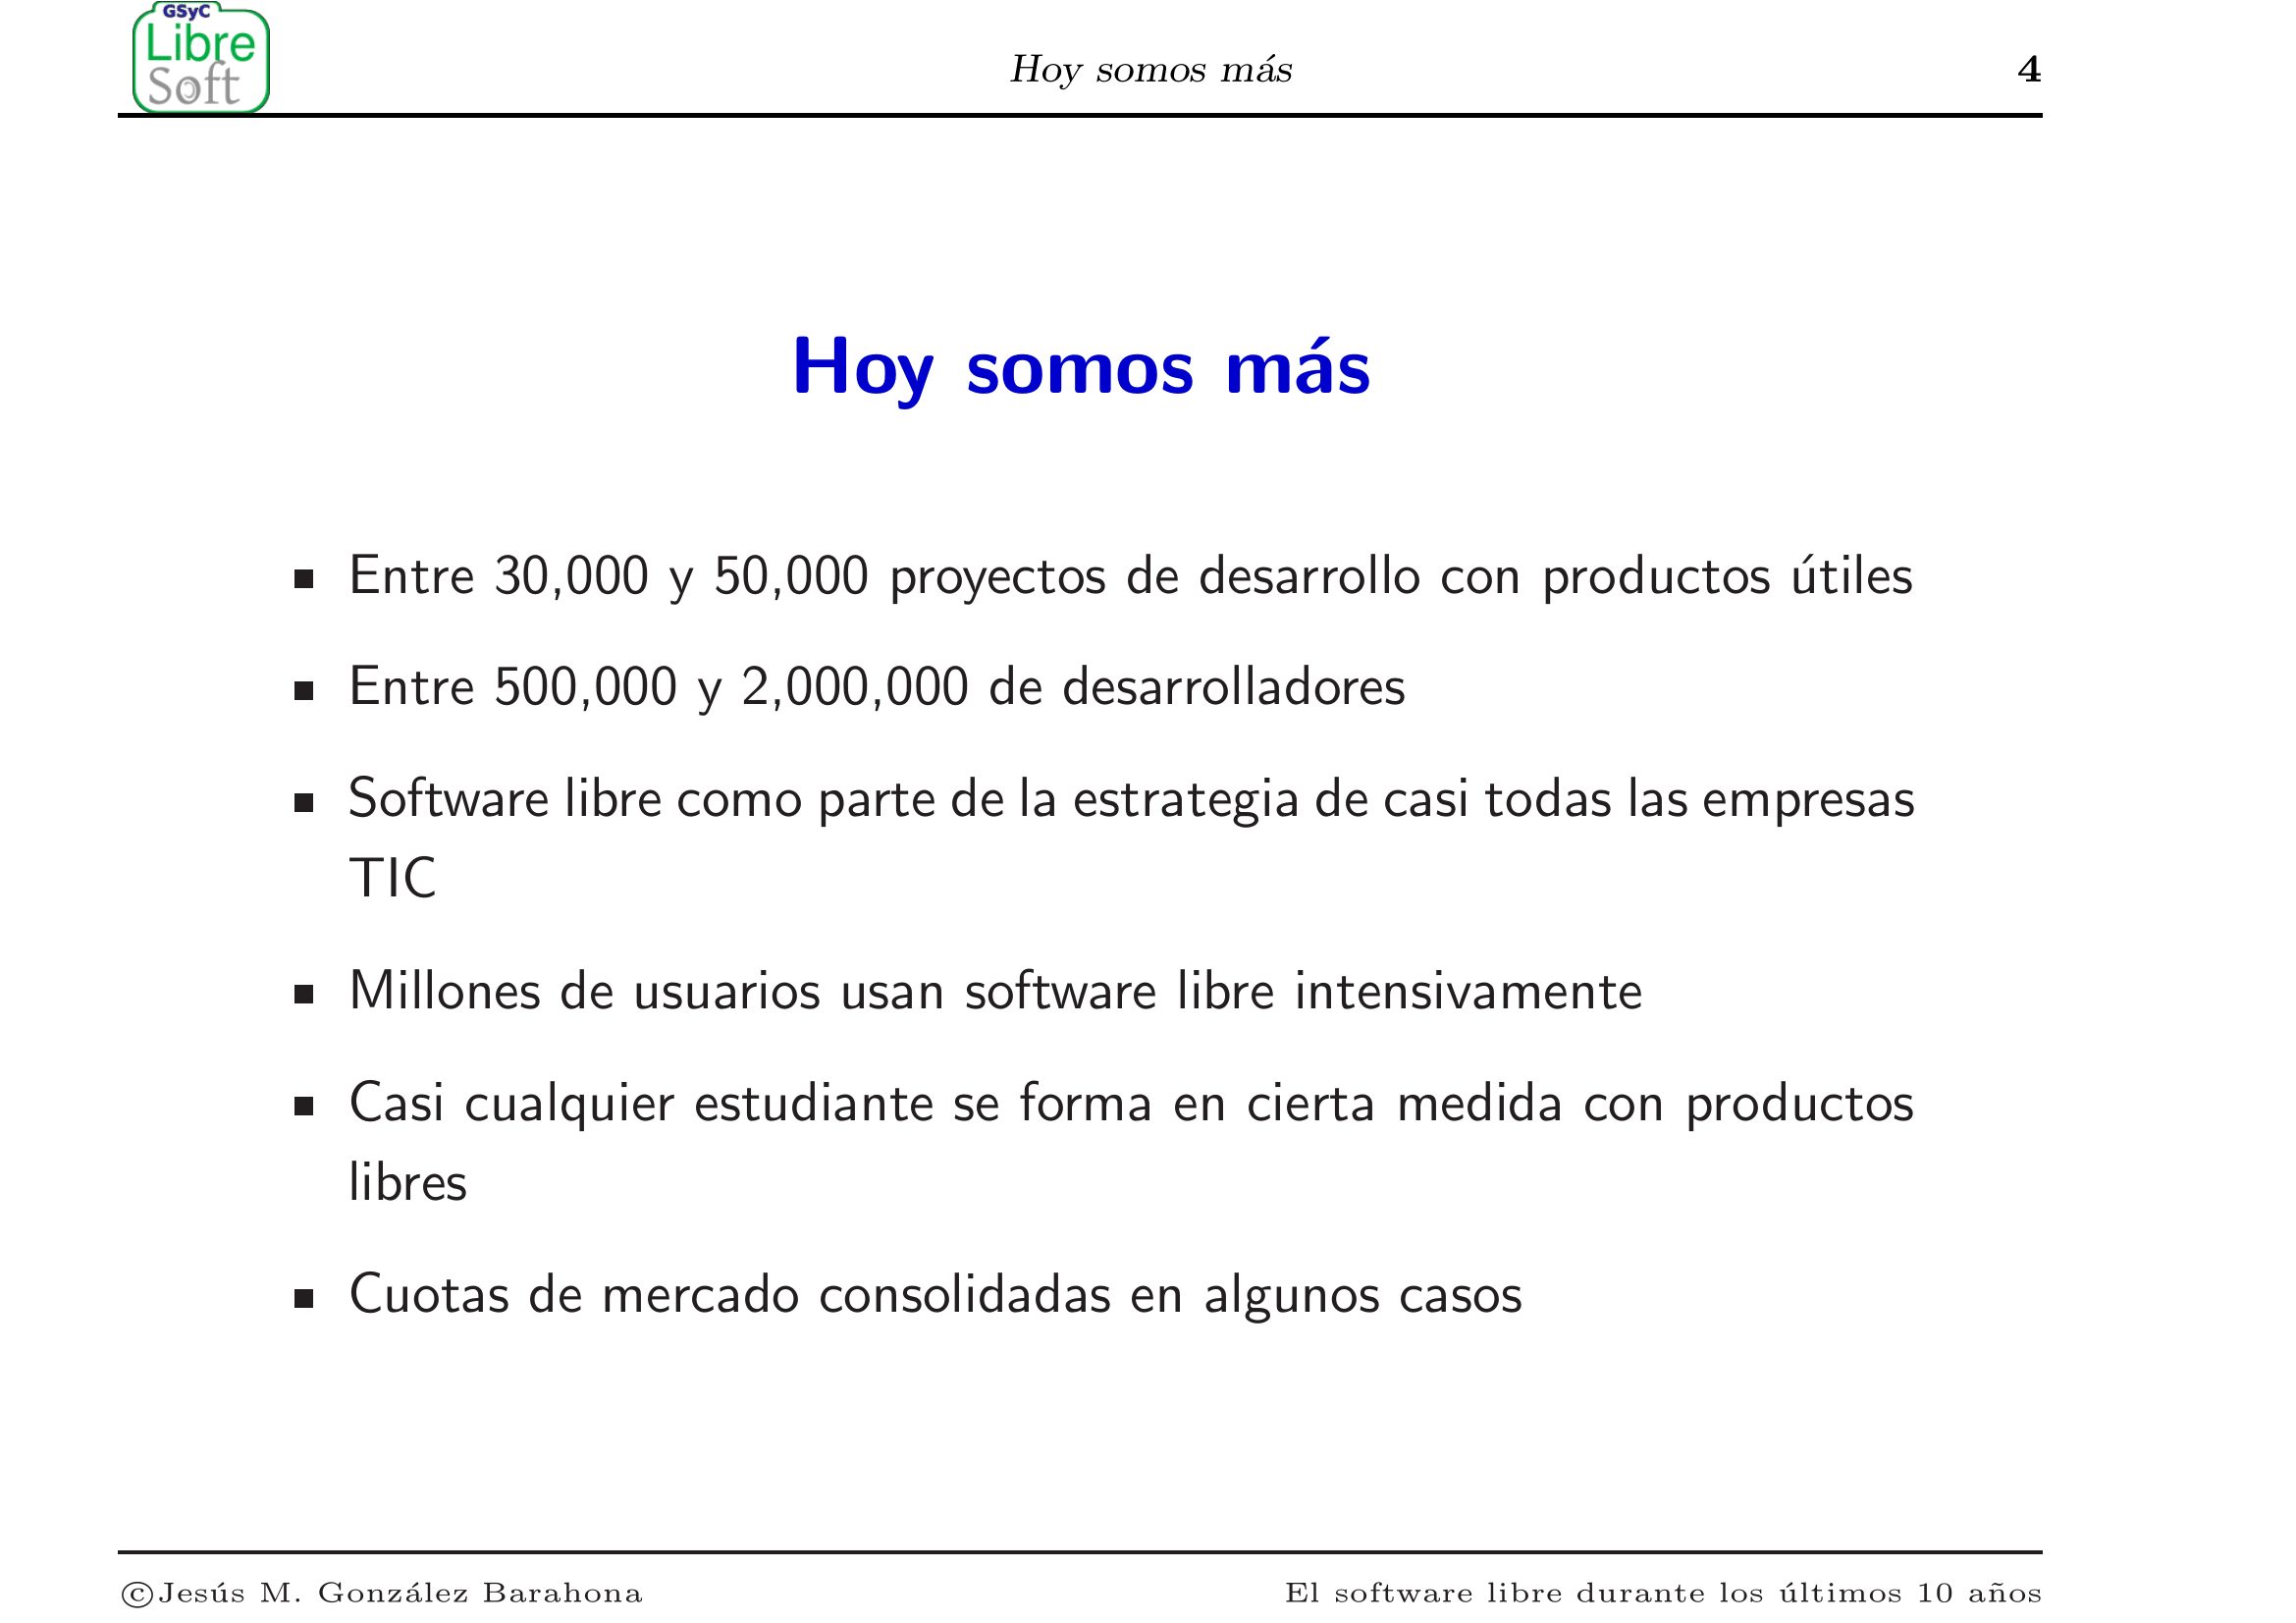
\includegraphics[width=12.5cm]{figs/transpas-05}
\end{center}  

\end{frame}

%%---------------------------------------------------------------
\begin{frame}
\frametitle{Hoy: por todas partes}

\begin{center}
  {\em \large
  El software libre se ha convertido \\
  en algo ubicuo... \\
  pero también, muchas veces \\
  invisible \\
  }
\end{center}  

\end{frame}

%%---------------------------------------------------------------
\begin{frame}
%\frametitle{}

\begin{center}
  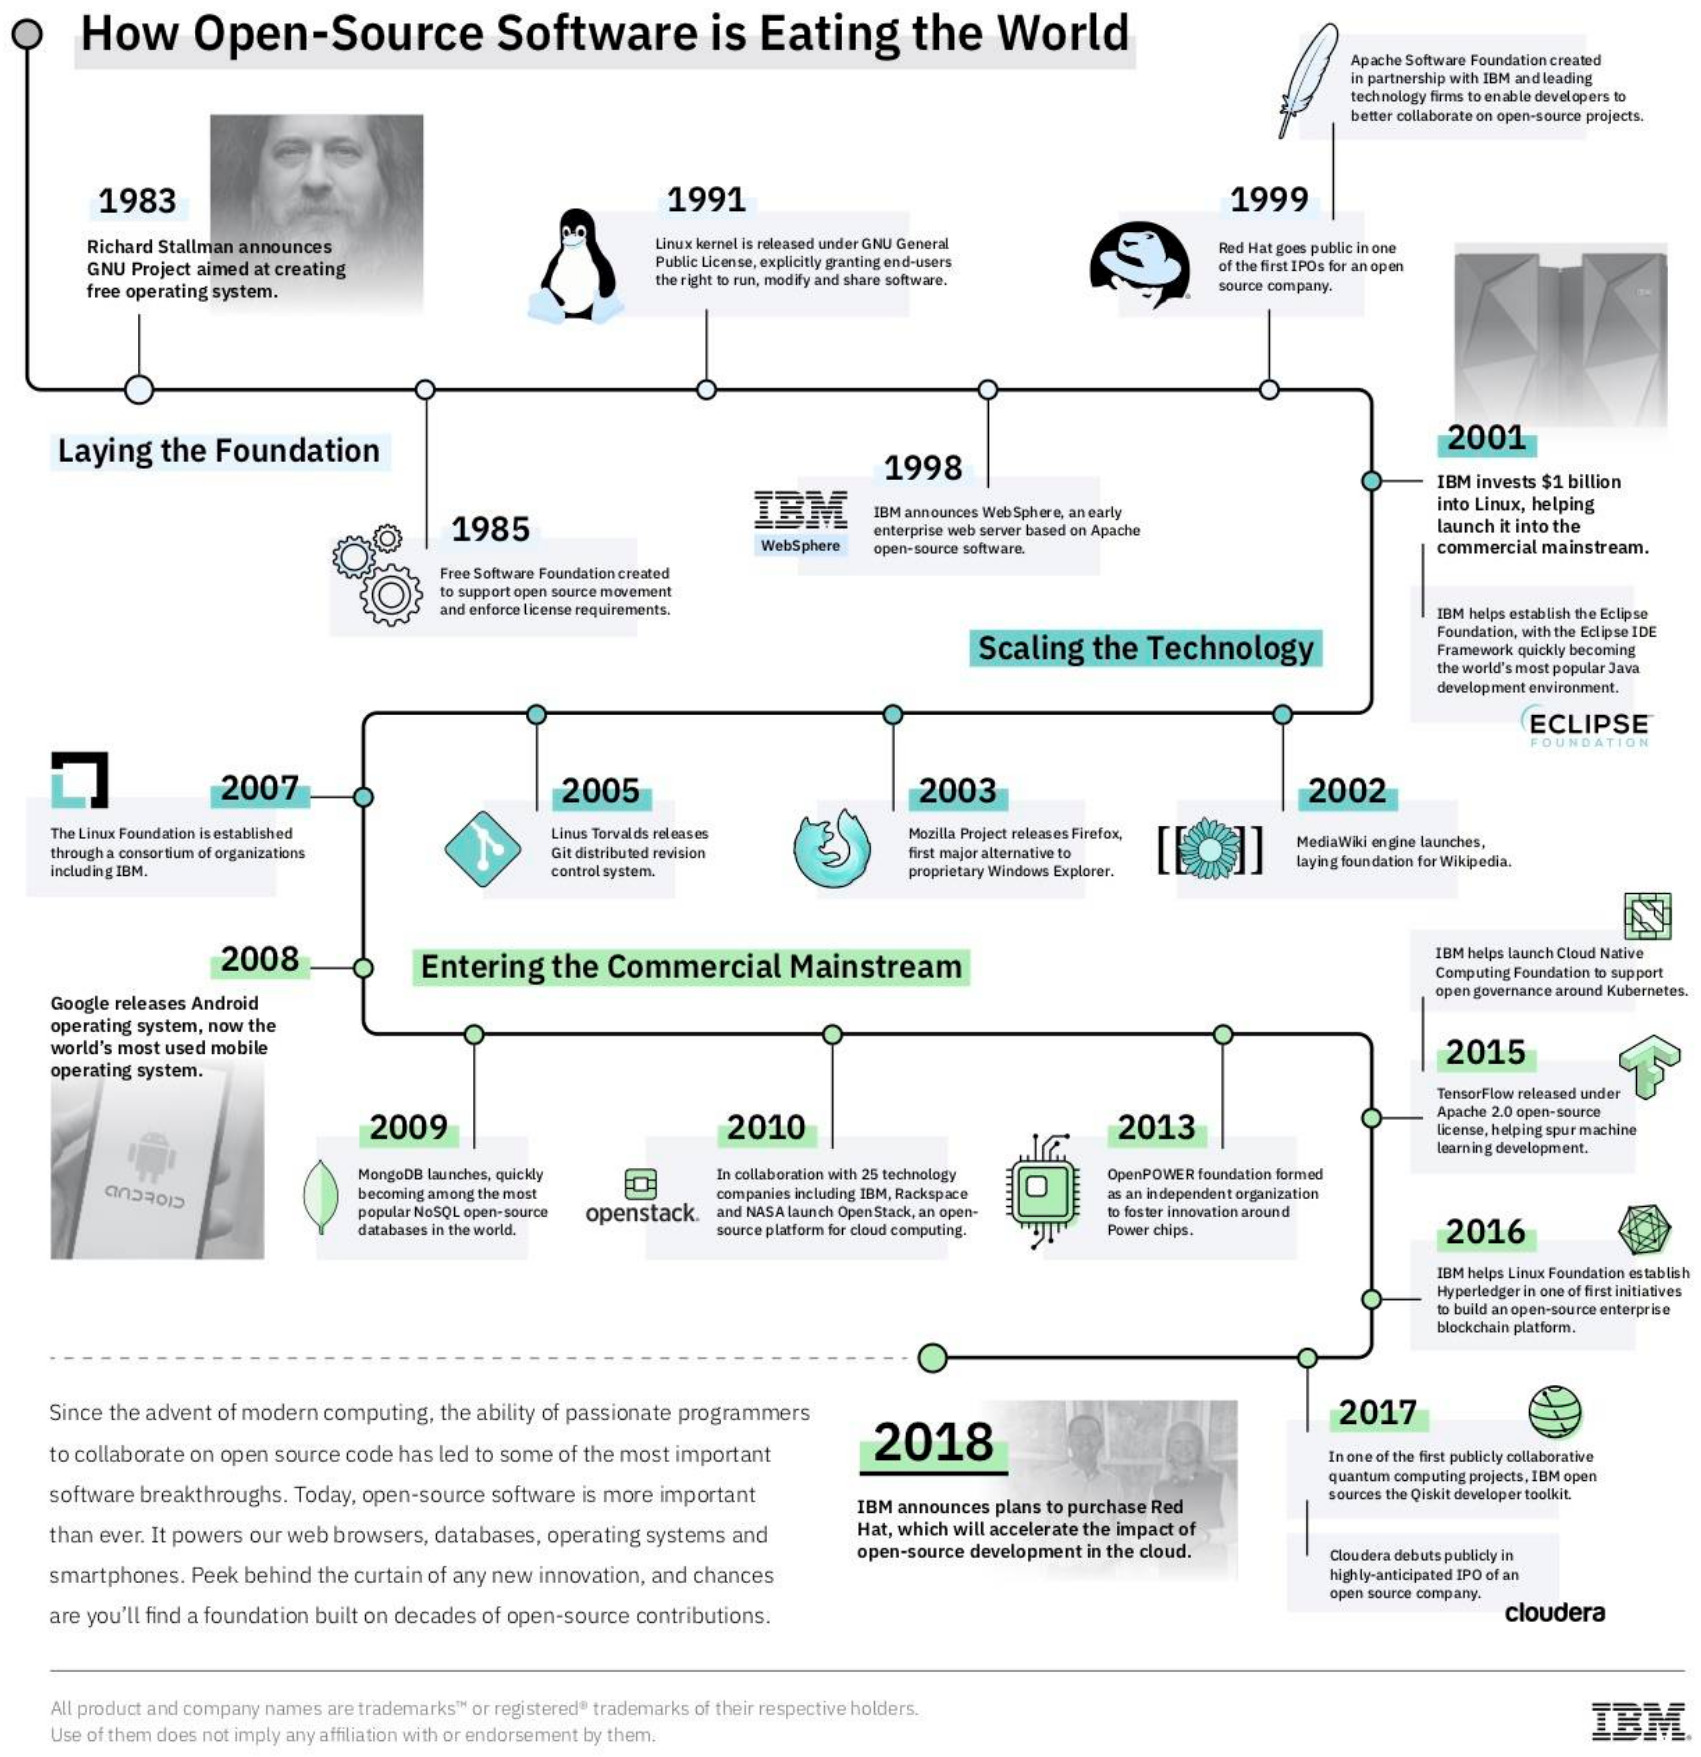
\includegraphics[height=7cm]{figs/ibm-opensource-eating-world}
\end{center}  

\begin{flushright}
  {\tiny{\url{https://developer.ibm.com/blogs/how-open-source-software-is-eating-the-world/}}}
\end{flushright}
\end{frame}

%%---------------------------------------------------------------

\begin{frame}

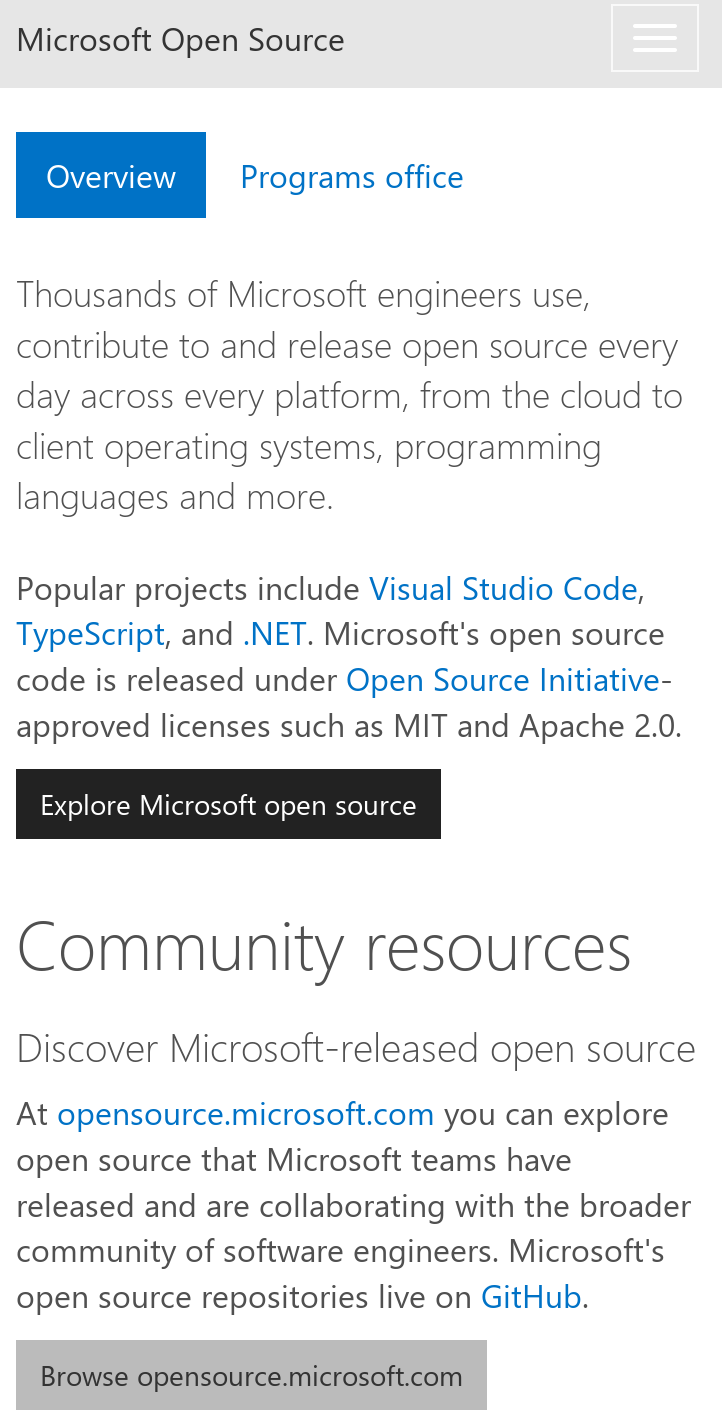
\includegraphics[width=.3\linewidth]{figs/microsoft-opensource}
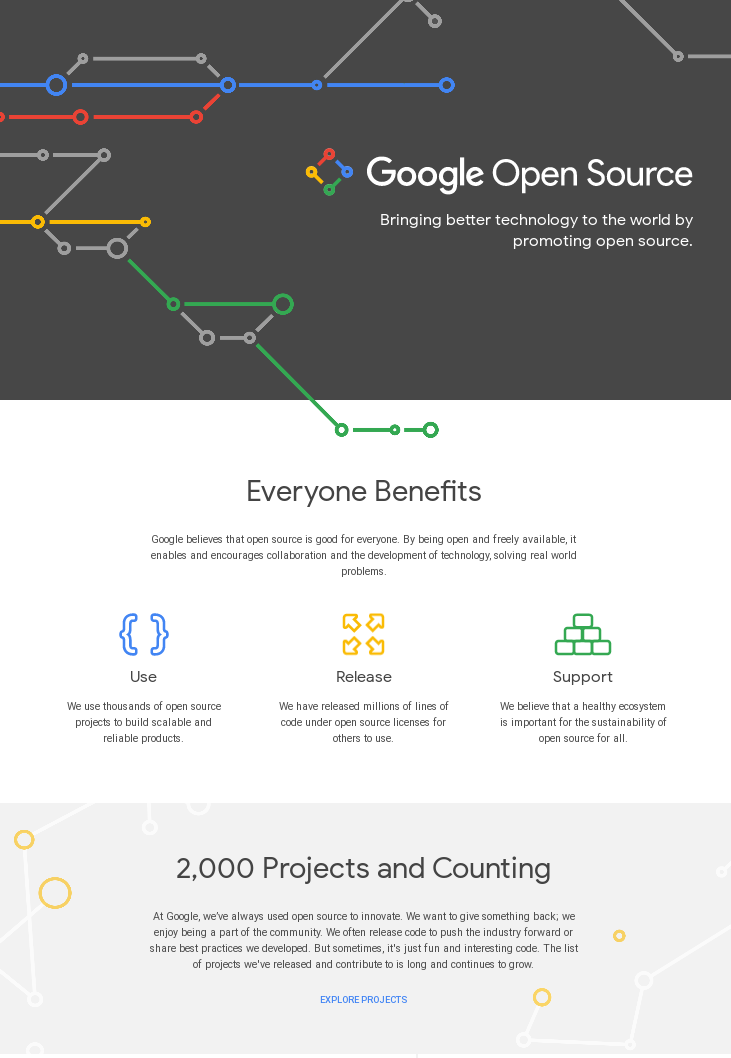
\includegraphics[width=.3\linewidth]{figs/google-opensource}
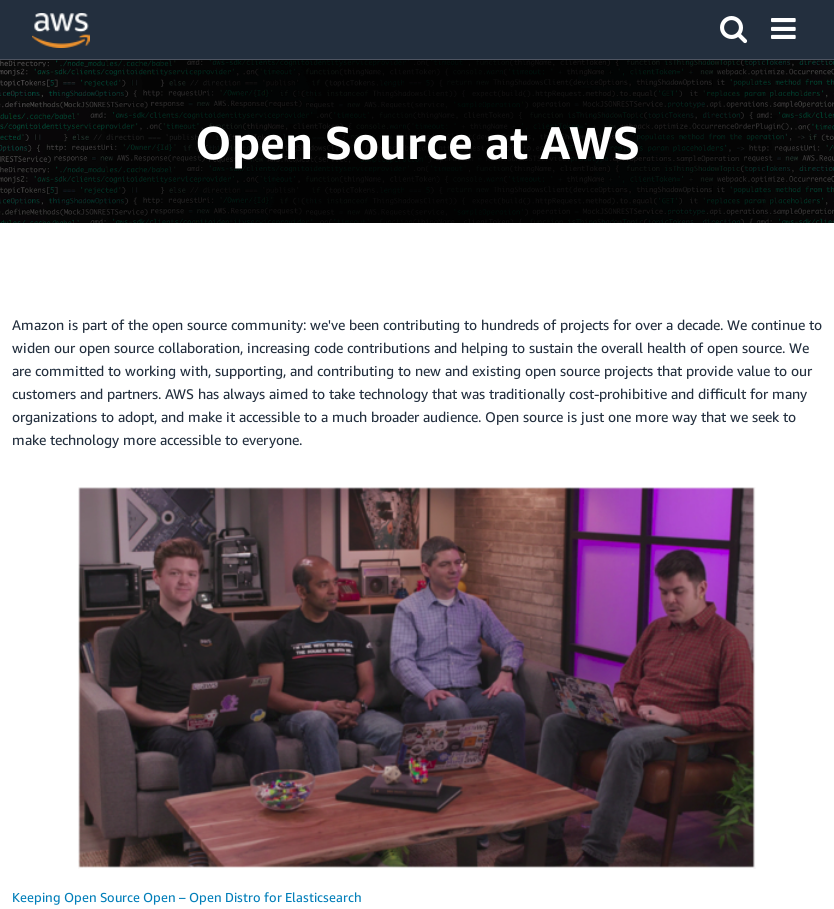
\includegraphics[width=.3\linewidth]{figs/aws-opensource}

\end{frame}

%%---------------------------------------------------------------
%%---------------------------------------------------------------
\section{Marcábamos tendencia}

%%---------------------------------------------------------------
\begin{frame}
%\frametitle{}

\begin{center}
  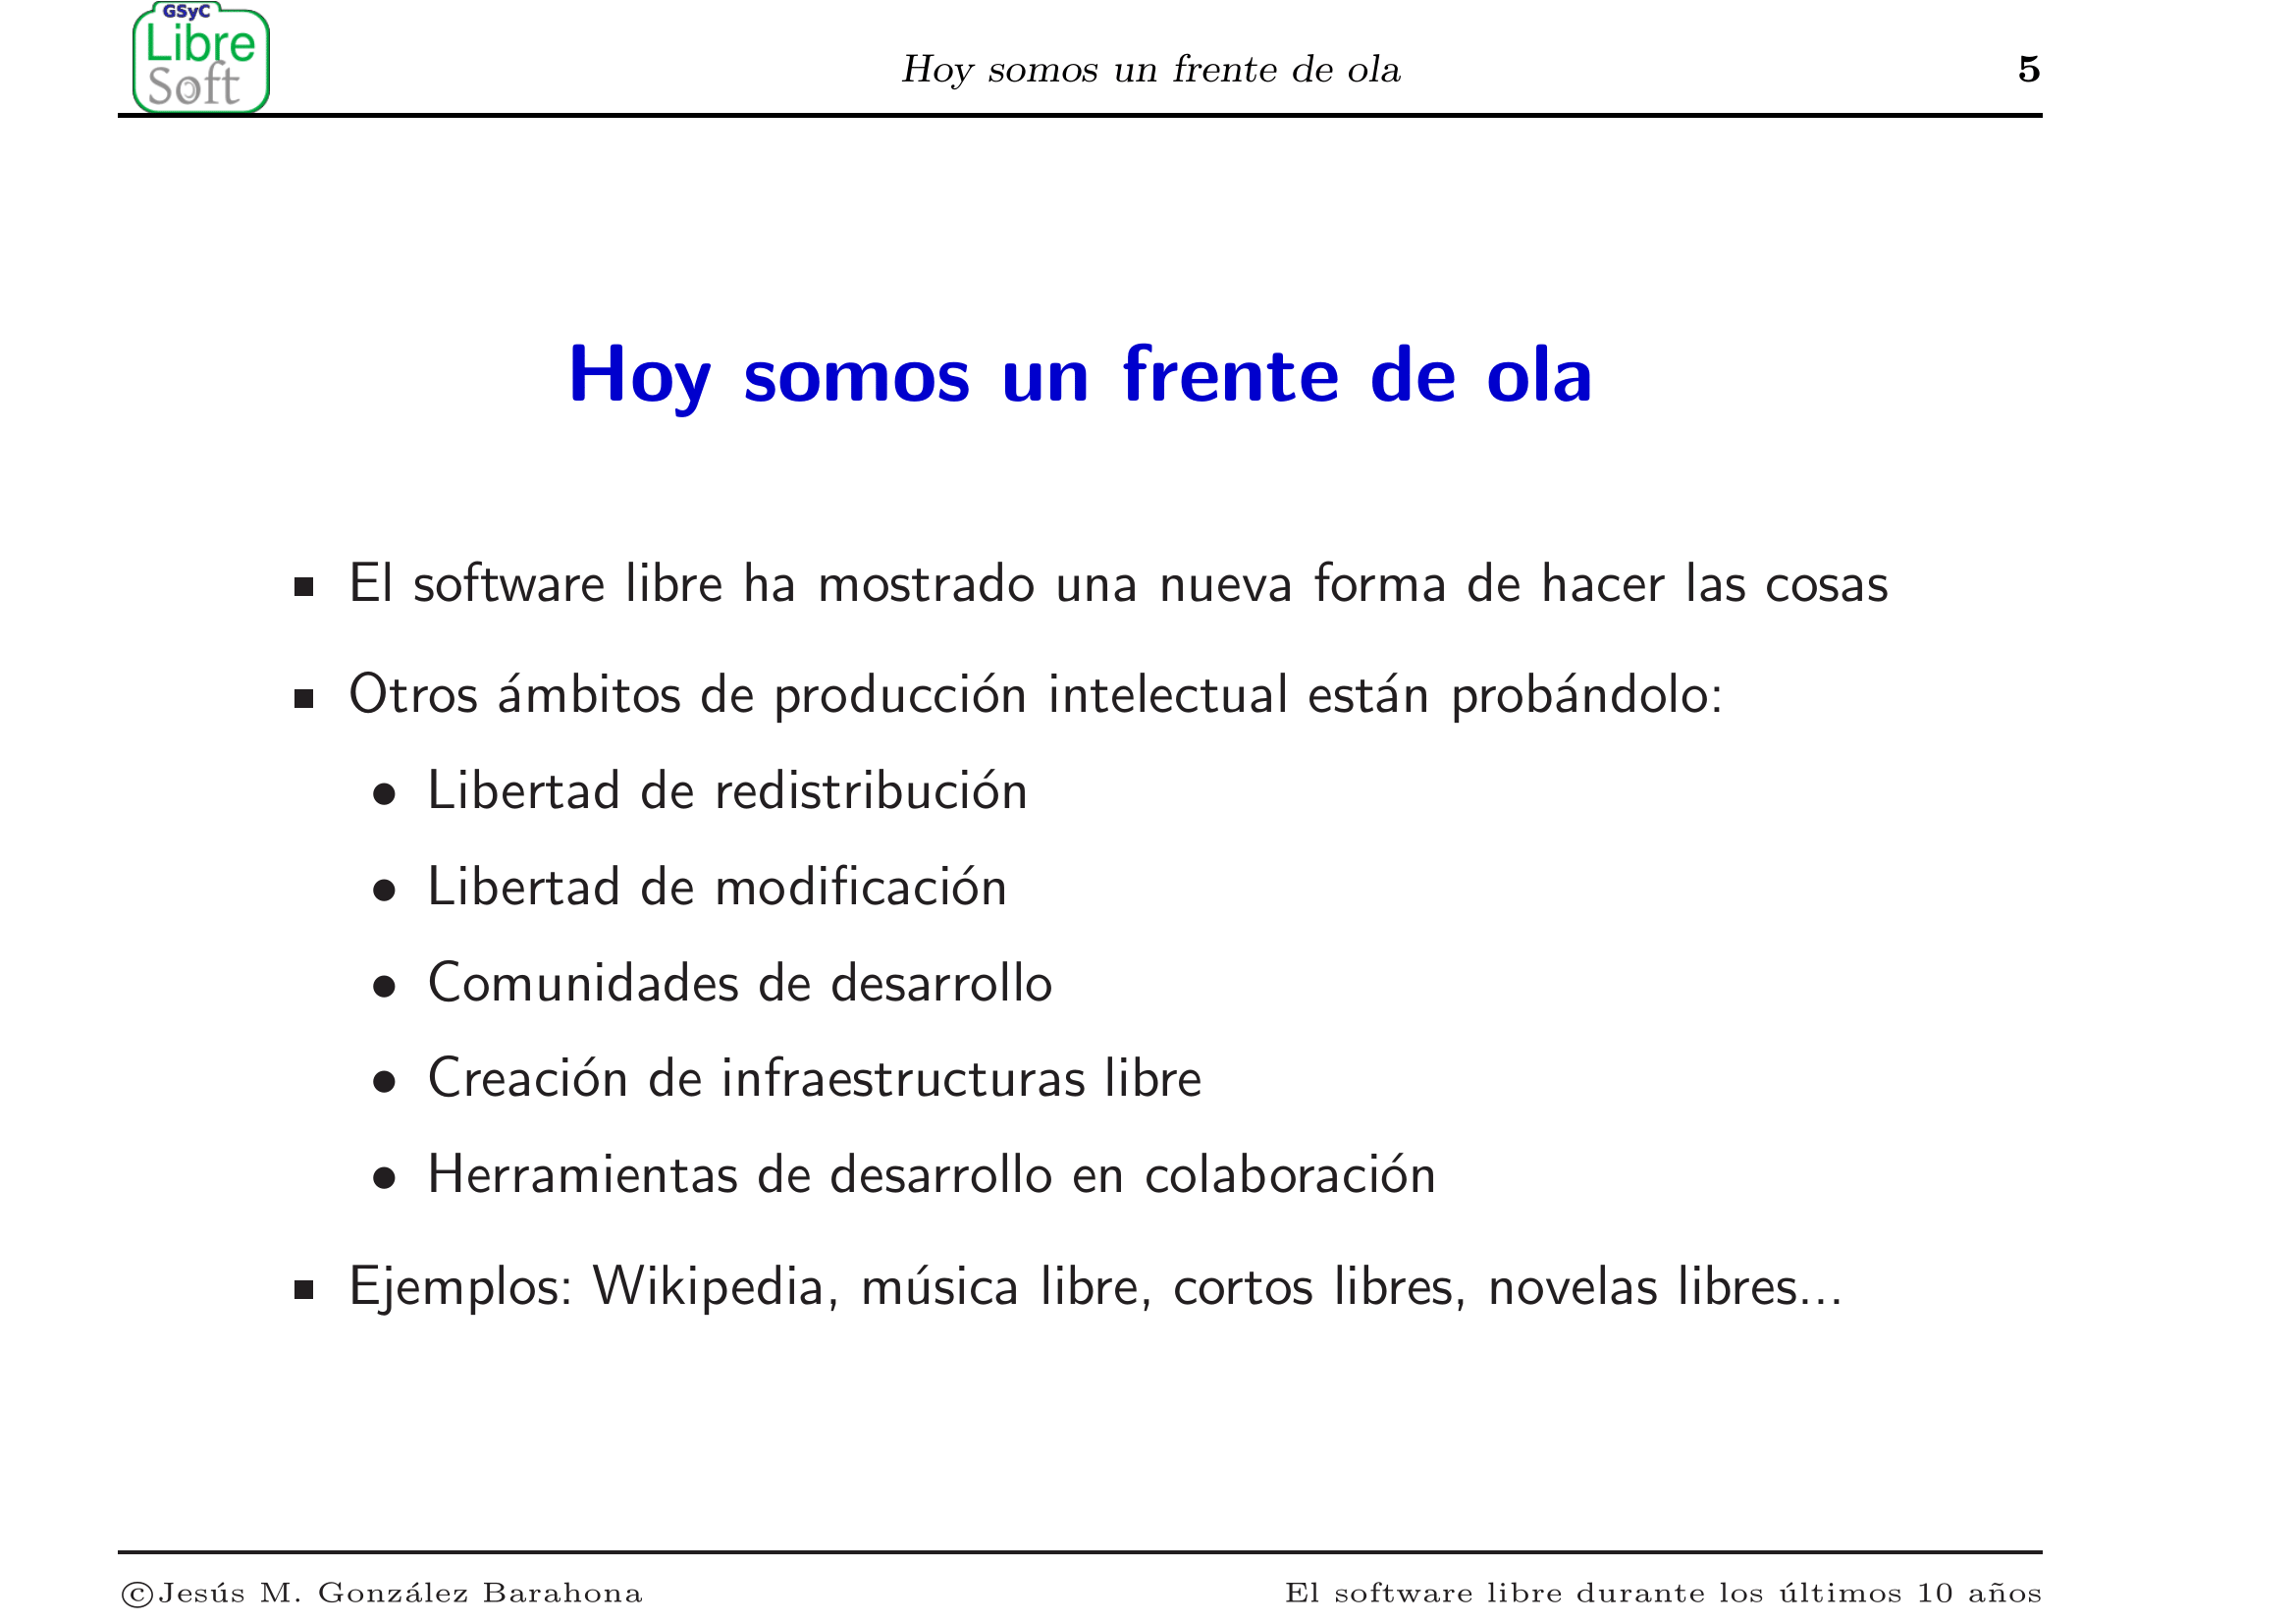
\includegraphics[width=12.5cm]{figs/transpas-06}
\end{center}  

\end{frame}

%%---------------------------------------------------------------
\begin{frame}
%\frametitle{}

  \begin{center}
    {\large
      ¿Hemos dejado de serlo? \\

      \vspace{1cm}
      
      ¿Seguimos cambiando el mundo? \\
    }
  \end{center}
  
\end{frame}

%%---------------------------------------------------------------
%%---------------------------------------------------------------
\section{Teníamos dudas}

%%---------------------------------------------------------------
\begin{frame}
%\frametitle{}

\begin{center}
  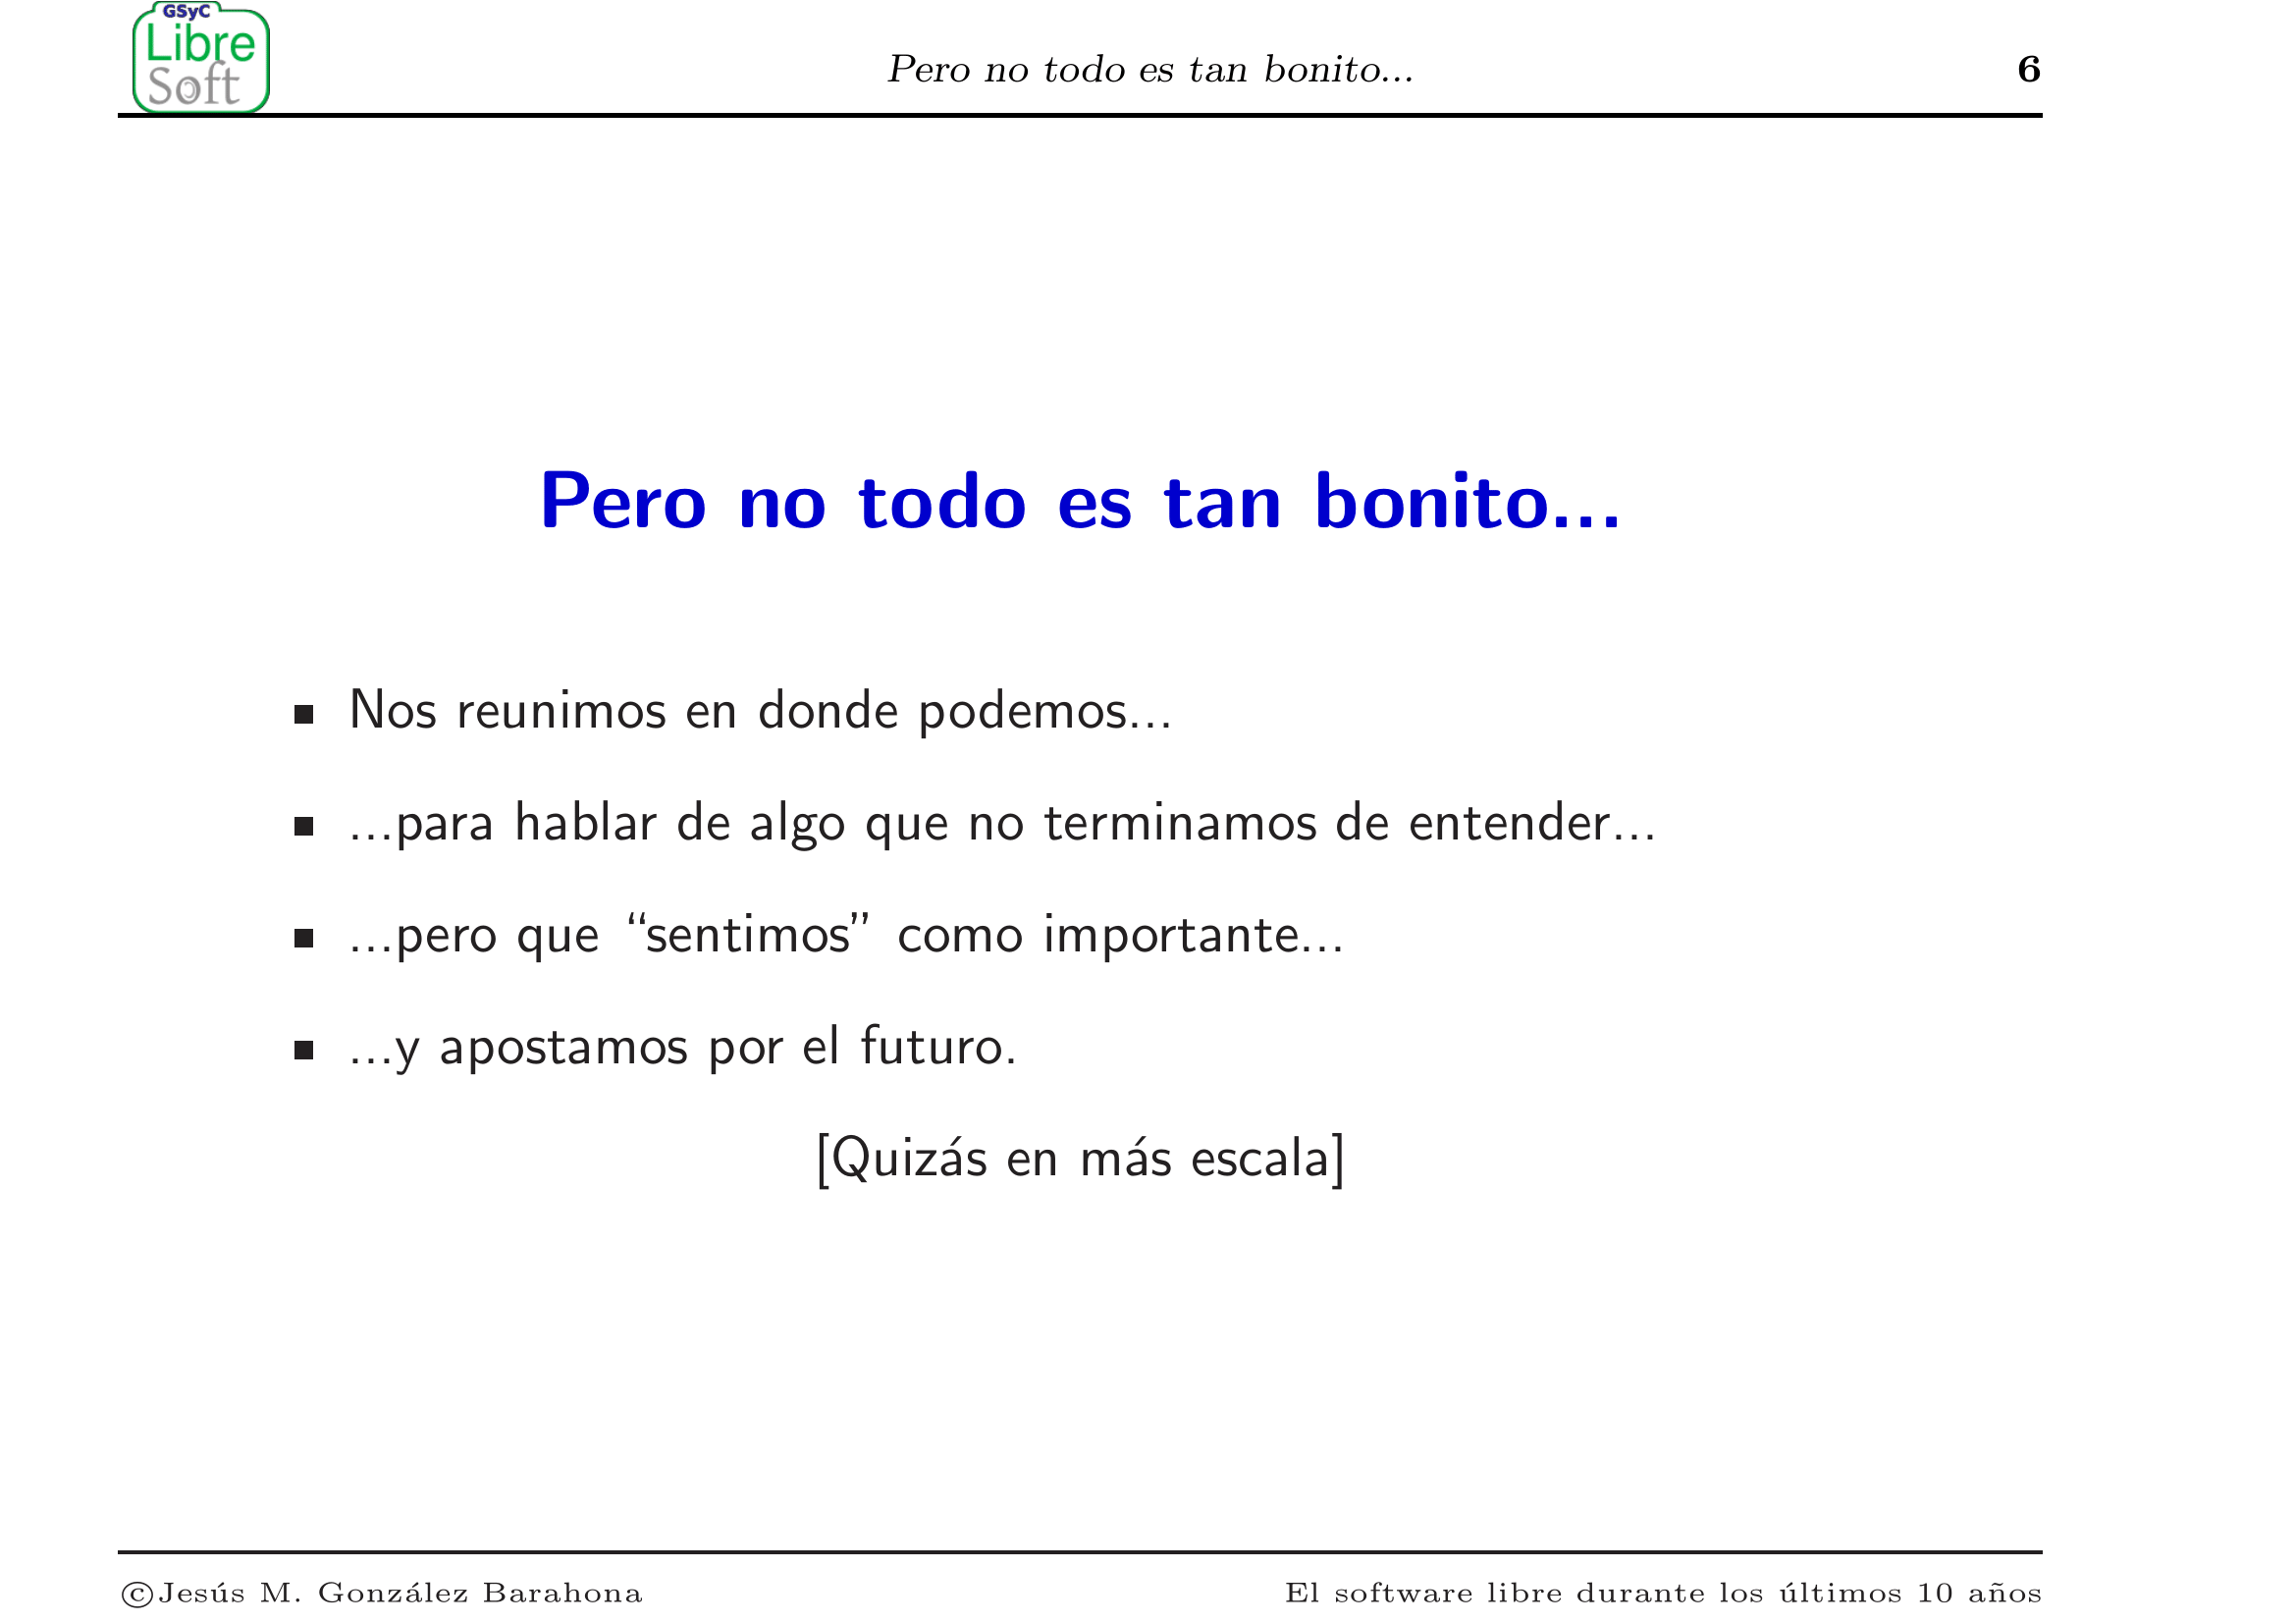
\includegraphics[width=12.5cm]{figs/transpas-07}
\end{center}  

\end{frame}

%%---------------------------------------------------------------
\begin{frame}
%\frametitle{}

  \begin{center}
    {\large
      ¿Hemos dejado de tener dudas...
      
      \vspace{1cm}
      
      ...porque ya no pensamos en ello? \\
    }
  \end{center}
  
\end{frame}

%%---------------------------------------------------------------
%%---------------------------------------------------------------
\section{Analizábamos}

%%---------------------------------------------------------------
\begin{frame}
%\frametitle{}

\begin{center}
  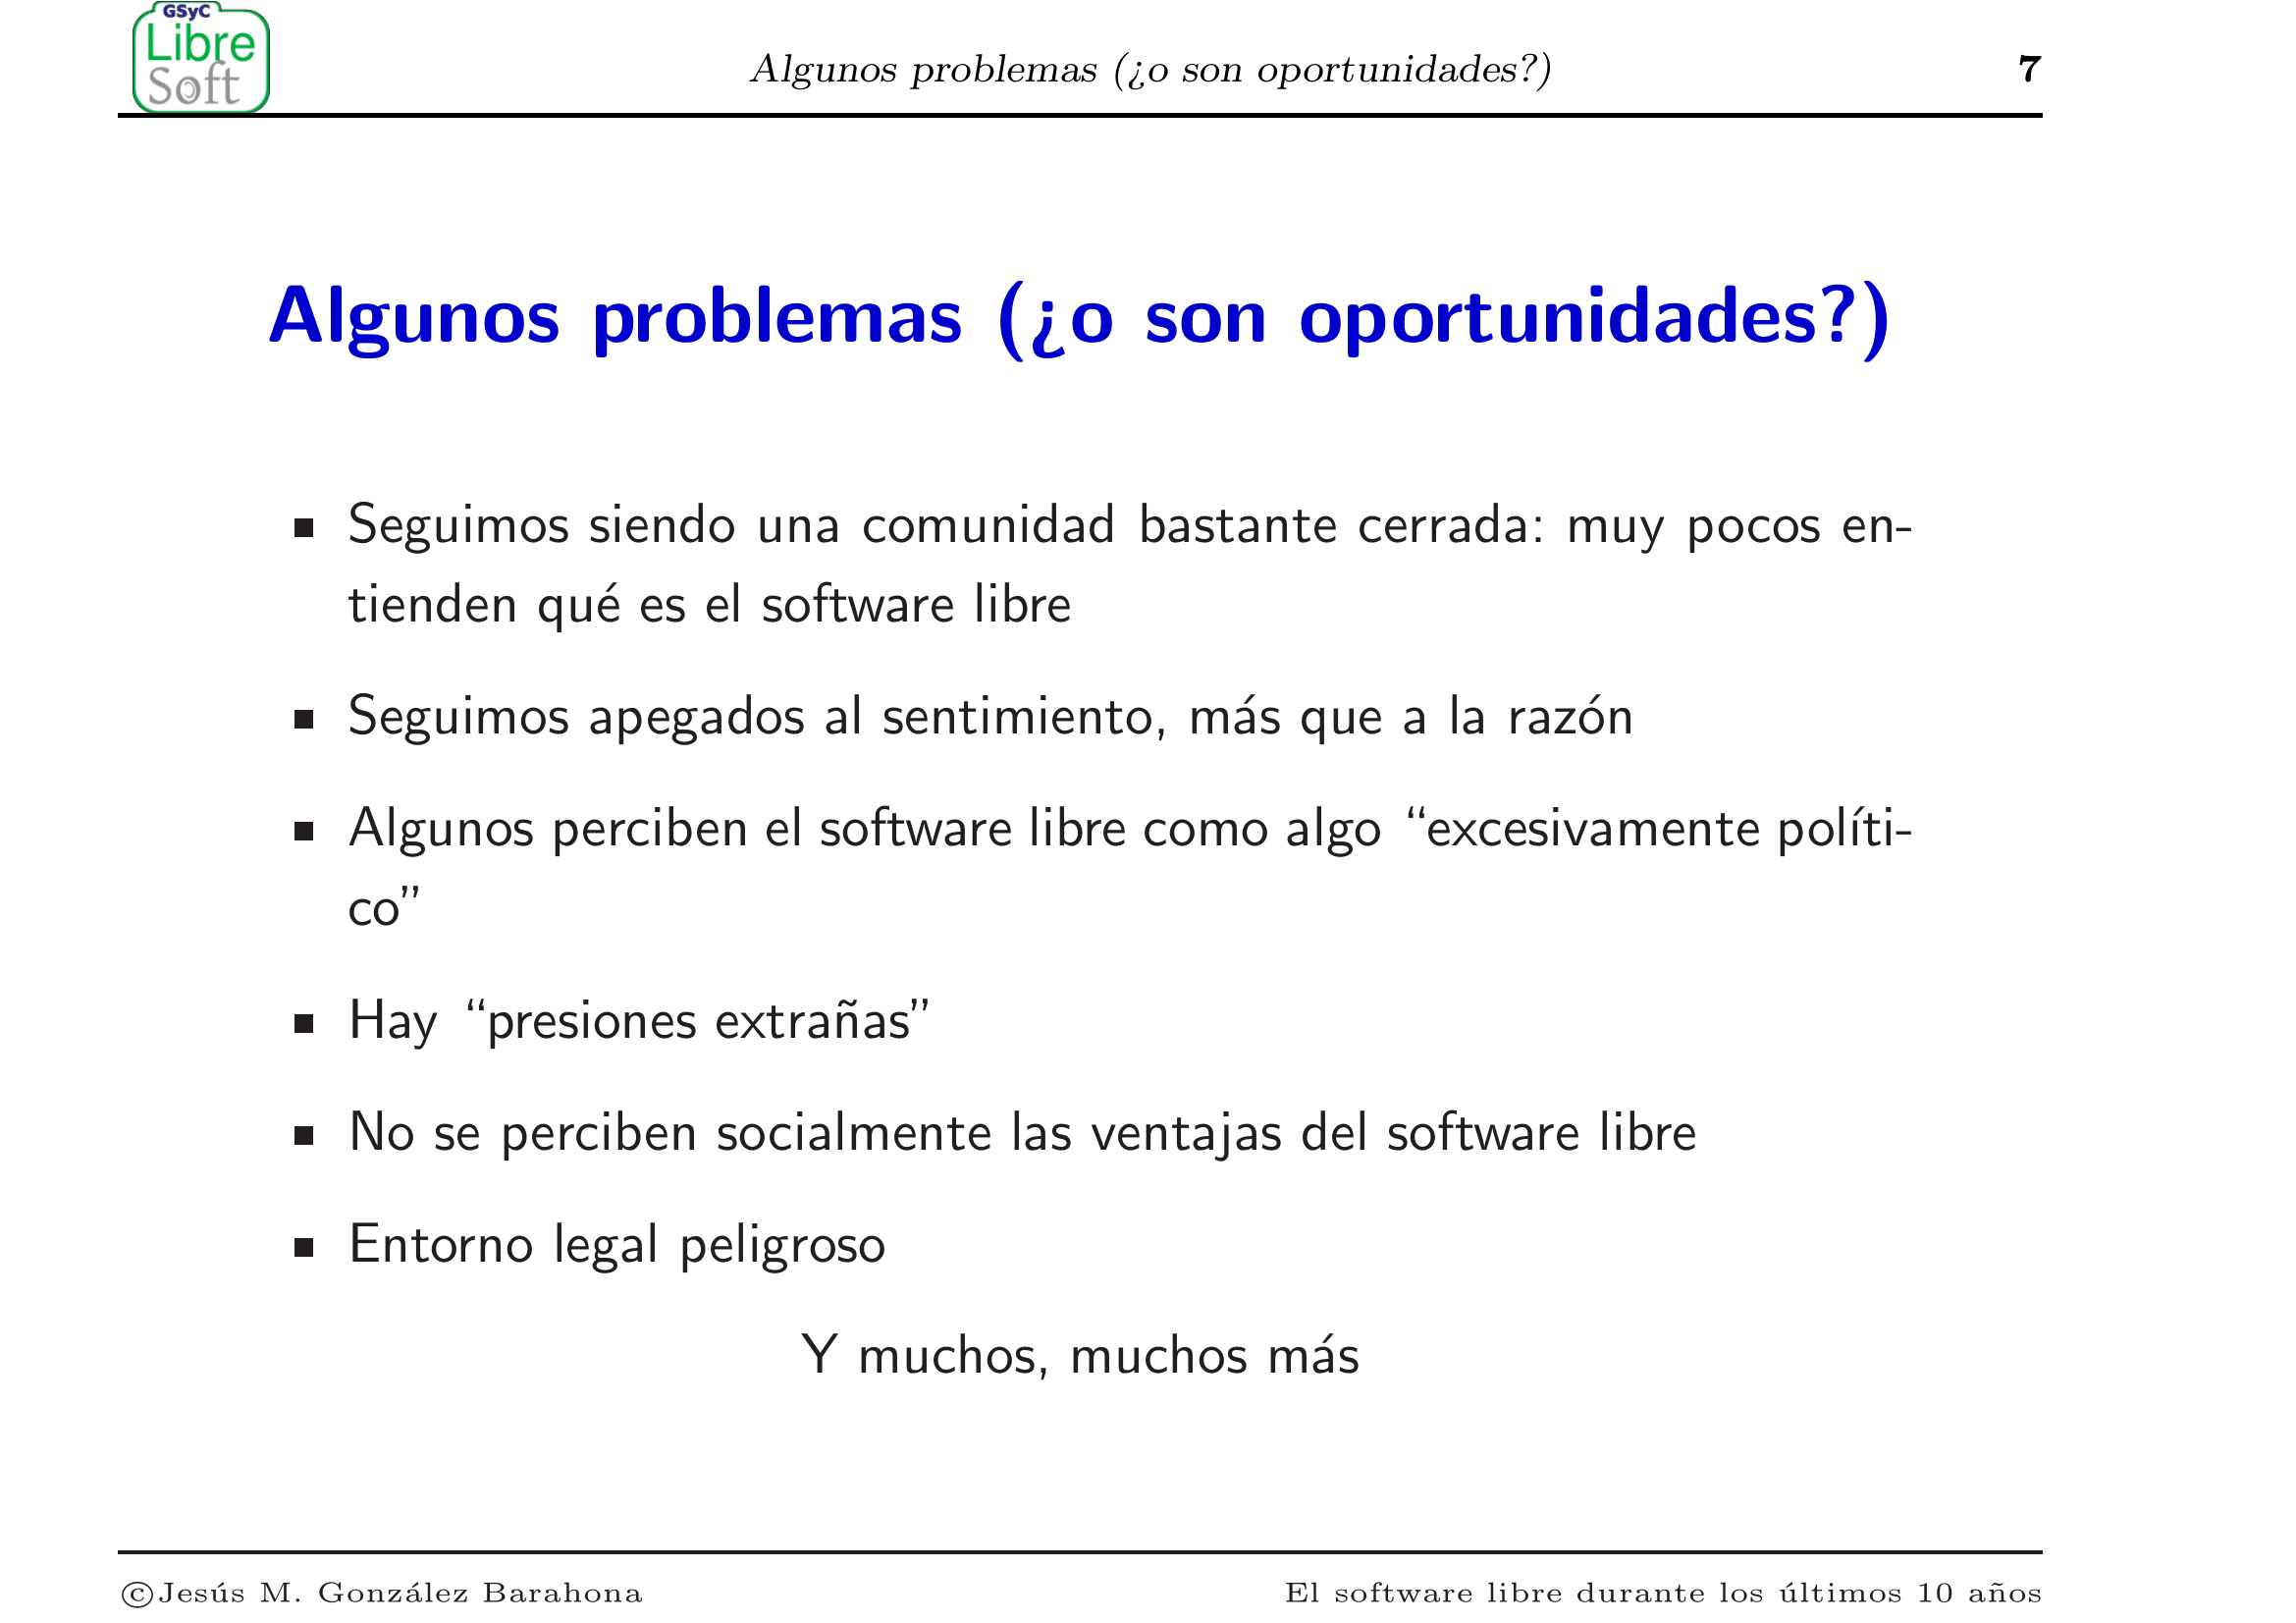
\includegraphics[width=12.5cm]{figs/transpas-08}
\end{center}  

\end{frame}

%%---------------------------------------------------------------
\begin{frame}
%\frametitle{}

  \begin{center}
    {\Large
      ¿Hemos resuelto alguno de ellos?
    }
  \end{center}
  
\end{frame}

%%---------------------------------------------------------------
%%---------------------------------------------------------------
\section{Soñábamos...}

%%---------------------------------------------------------------
\begin{frame}
%\frametitle{}

\begin{center}
  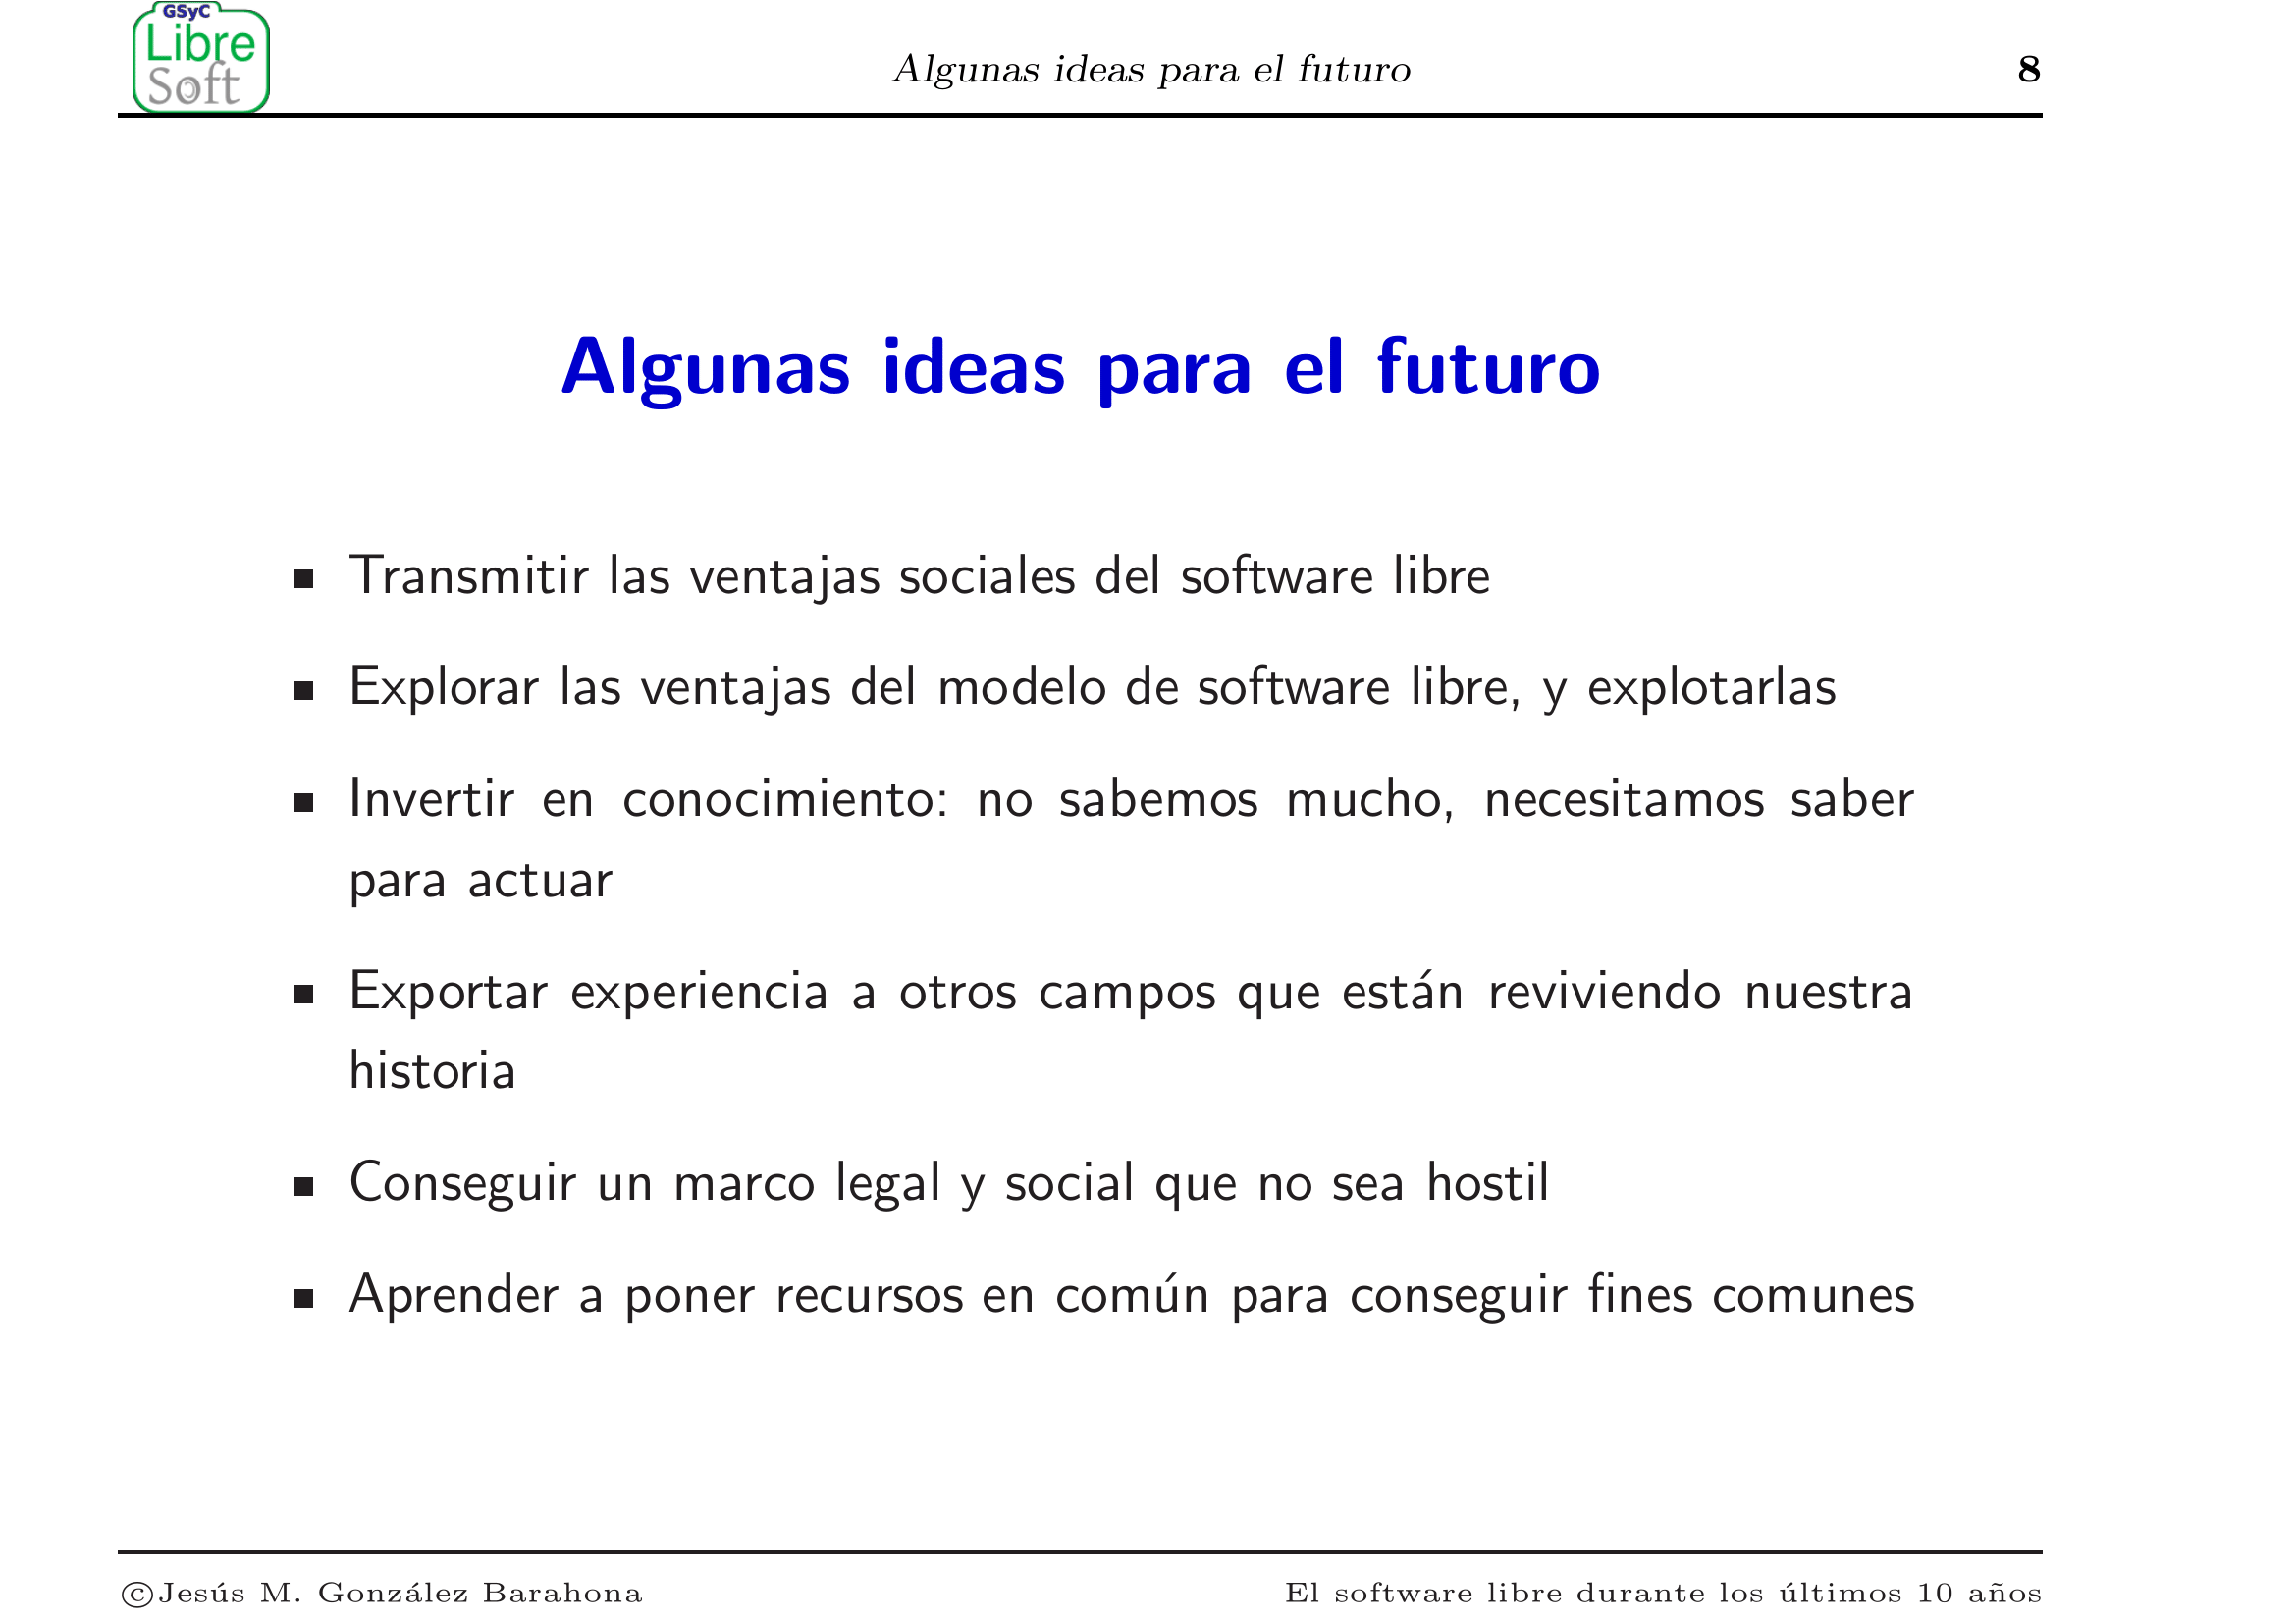
\includegraphics[width=12.5cm]{figs/transpas-09}
\end{center}  

\end{frame}

%%---------------------------------------------------------------
\begin{frame}
%\frametitle{}

  \begin{center}
    {\large
      Ya estamos en el futuro \\
      \vspace{1cm}

      ¿Estamos en ese futuro? \\
    }
  \end{center}
  
\end{frame}

%%---------------------------------------------------------------
%%---------------------------------------------------------------
\section{Teníamos planes}

%%---------------------------------------------------------------
\begin{frame}
%\frametitle{}

\begin{center}
  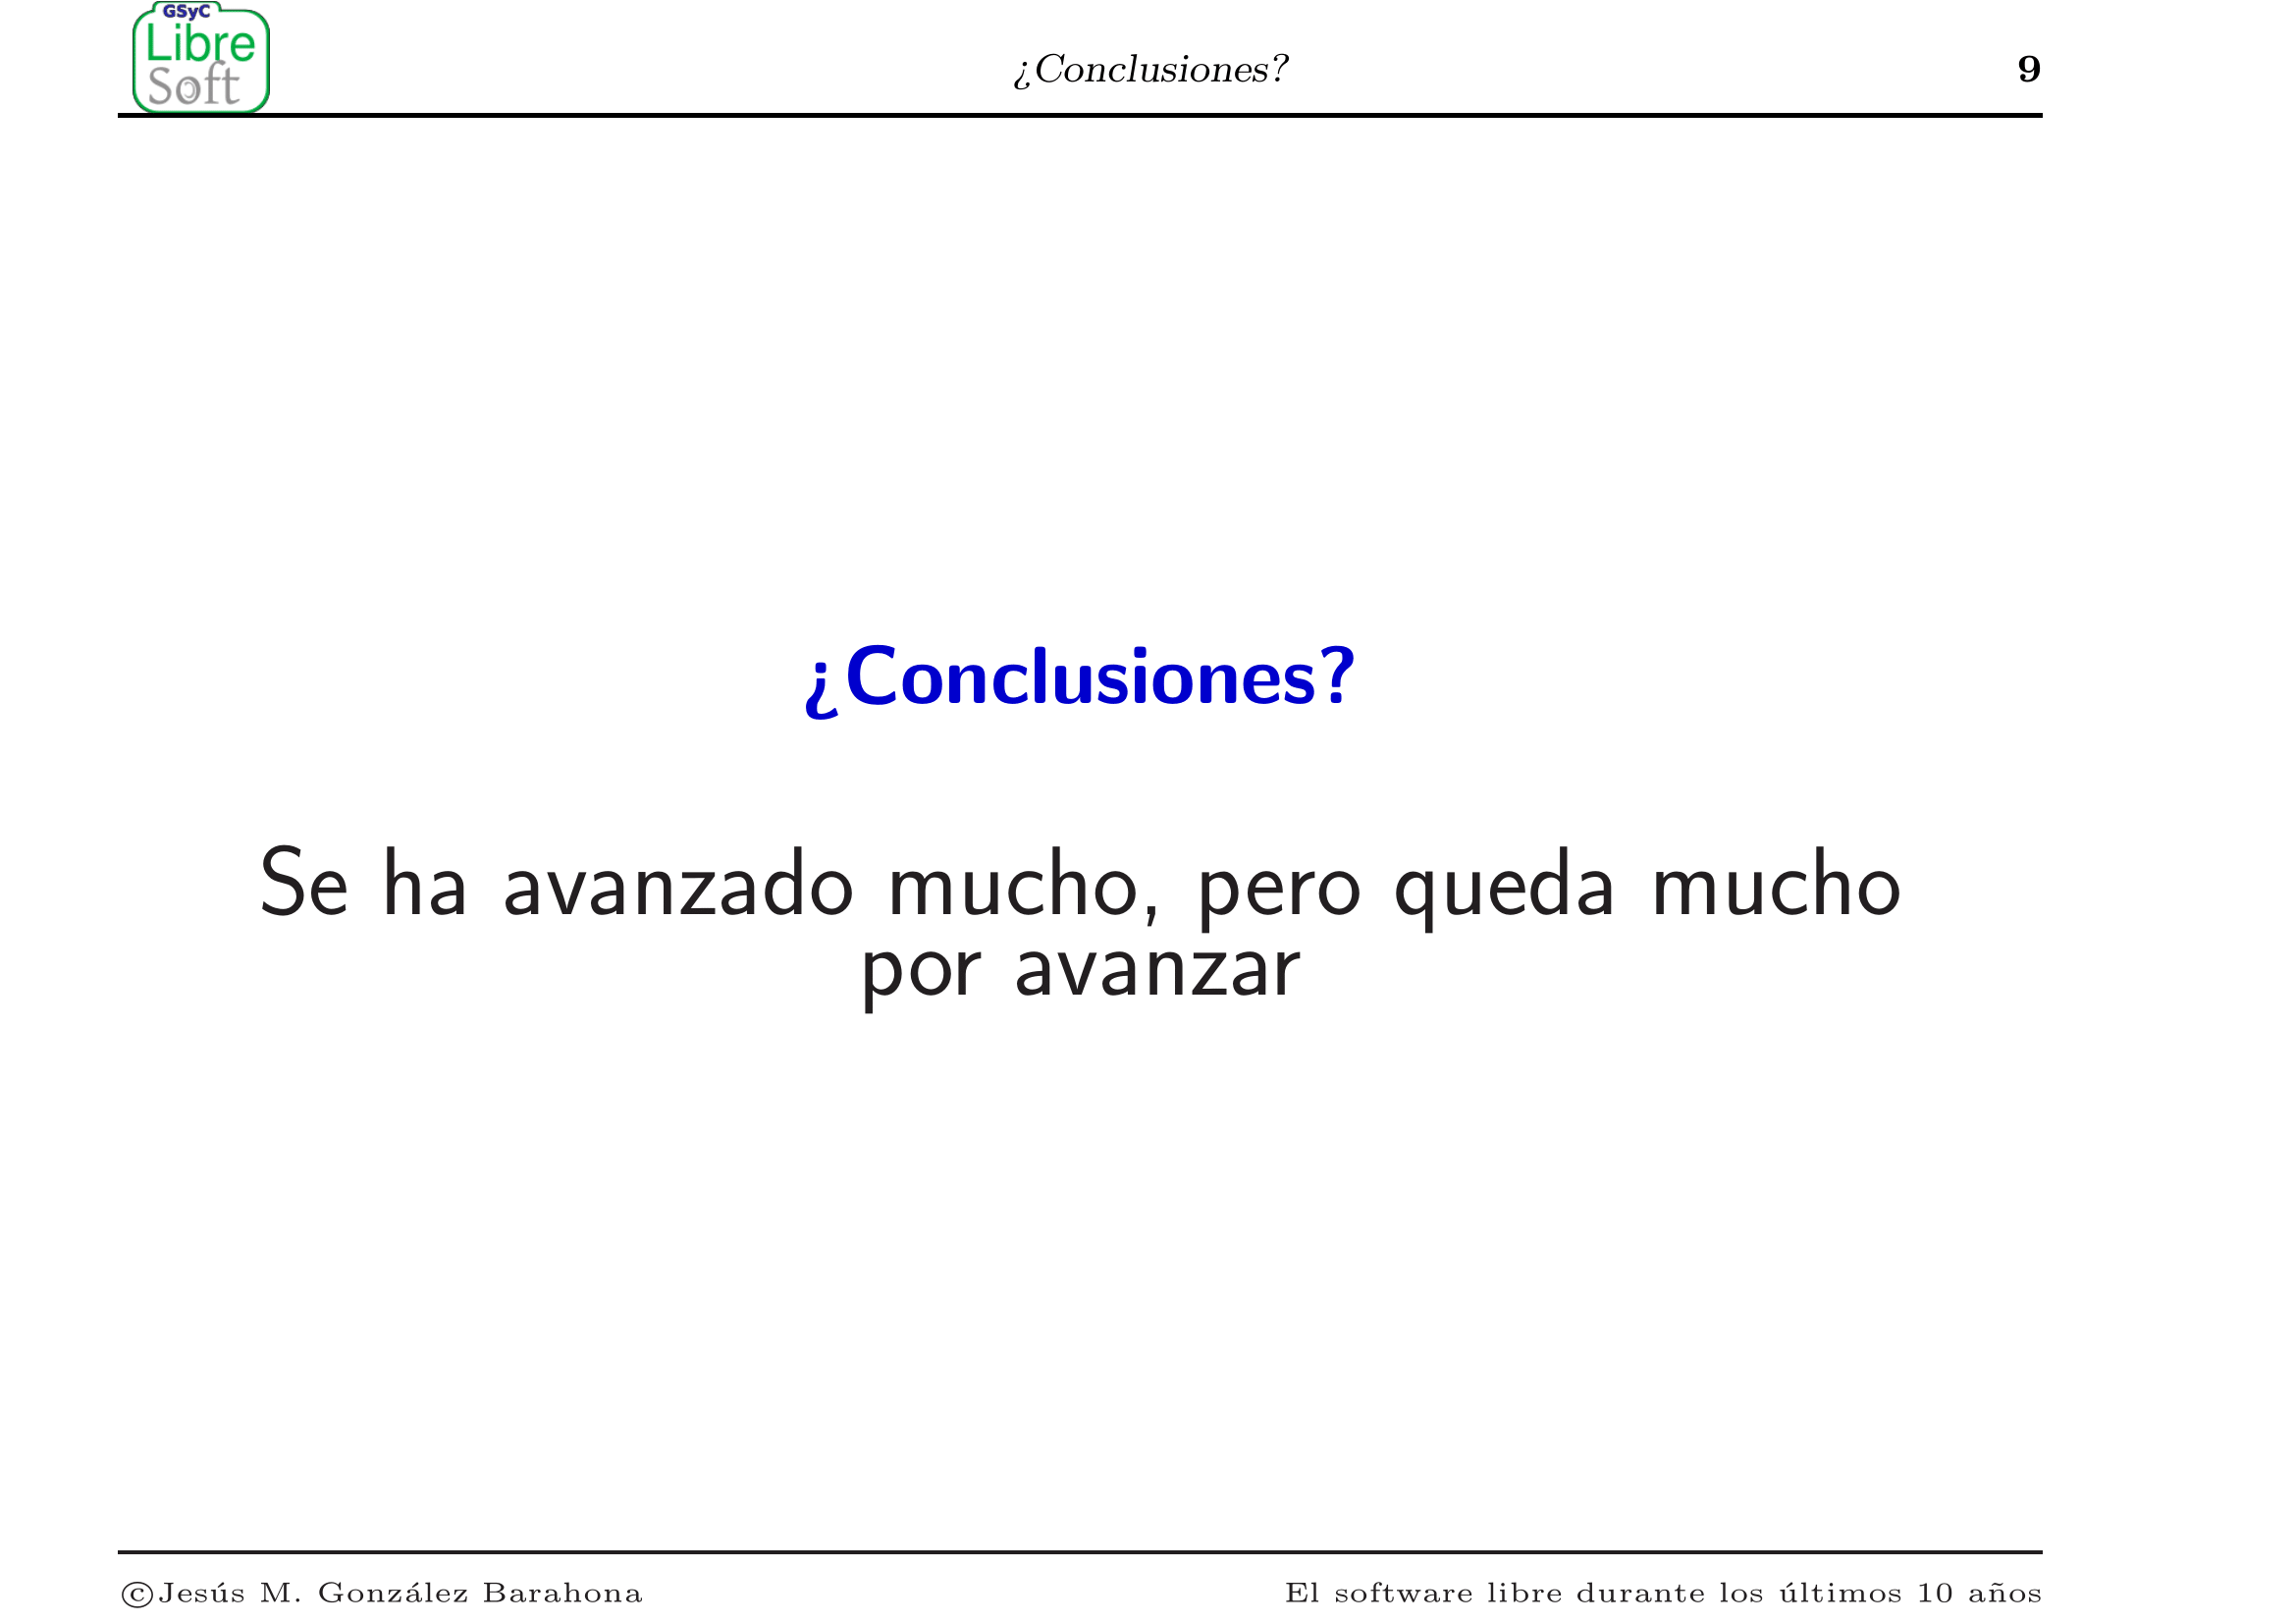
\includegraphics[width=12.5cm]{figs/transpas-10}
\end{center}  

\end{frame}

%%---------------------------------------------------------------
\begin{frame}
%\frametitle{}

  \begin{center}
    {\Large
      ¿Necesitamos nuevos planes?
    }
  \end{center}
  
\end{frame}

%%---------------------------------------------------------------
%%---------------------------------------------------------------
\section{Lo que no ha cambiado}

%%---------------------------------------------------------------

\begin{frame}
\frametitle{El software libre permite...}

{\large
\begin{itemize}
\item usarlo como mejor te parezca
\item redistribuirlo a quien quieras
\item modificarlo (mejorarlo, adaptarlo)
\item redistribuir las modificaciones
\end{itemize}
}
\end{frame}

%%---------------------------------------------------------------

\begin{frame}

  {\large
    Hace más de 30 años \\
    un grupo de visionarios \\
    decidieron que tenían \\
    que cambiar el mundo
  }

  \begin{flushright}
    {\huge
      Y lo cambiaron
    }
  \end{flushright}
\end{frame}

%%---------------------------------------------------------------

\begin{frame}
  \frametitle{En la década de 2020...}
  
  {\Large
    El software va a mediar \\
    todo lo que hacemos, \\
    todo lo que somos \\
  }

\end{frame}

%%---------------------------------------------------------------

\begin{frame}
  
  \begin{center}
    {\em \huge
      Tenemos trabajo \\
      que hacer... \\
    }
  \end{center}
\end{frame}

%%---------------------------------------------------------------
\begin{frame}
%\frametitle{}

\begin{center}
  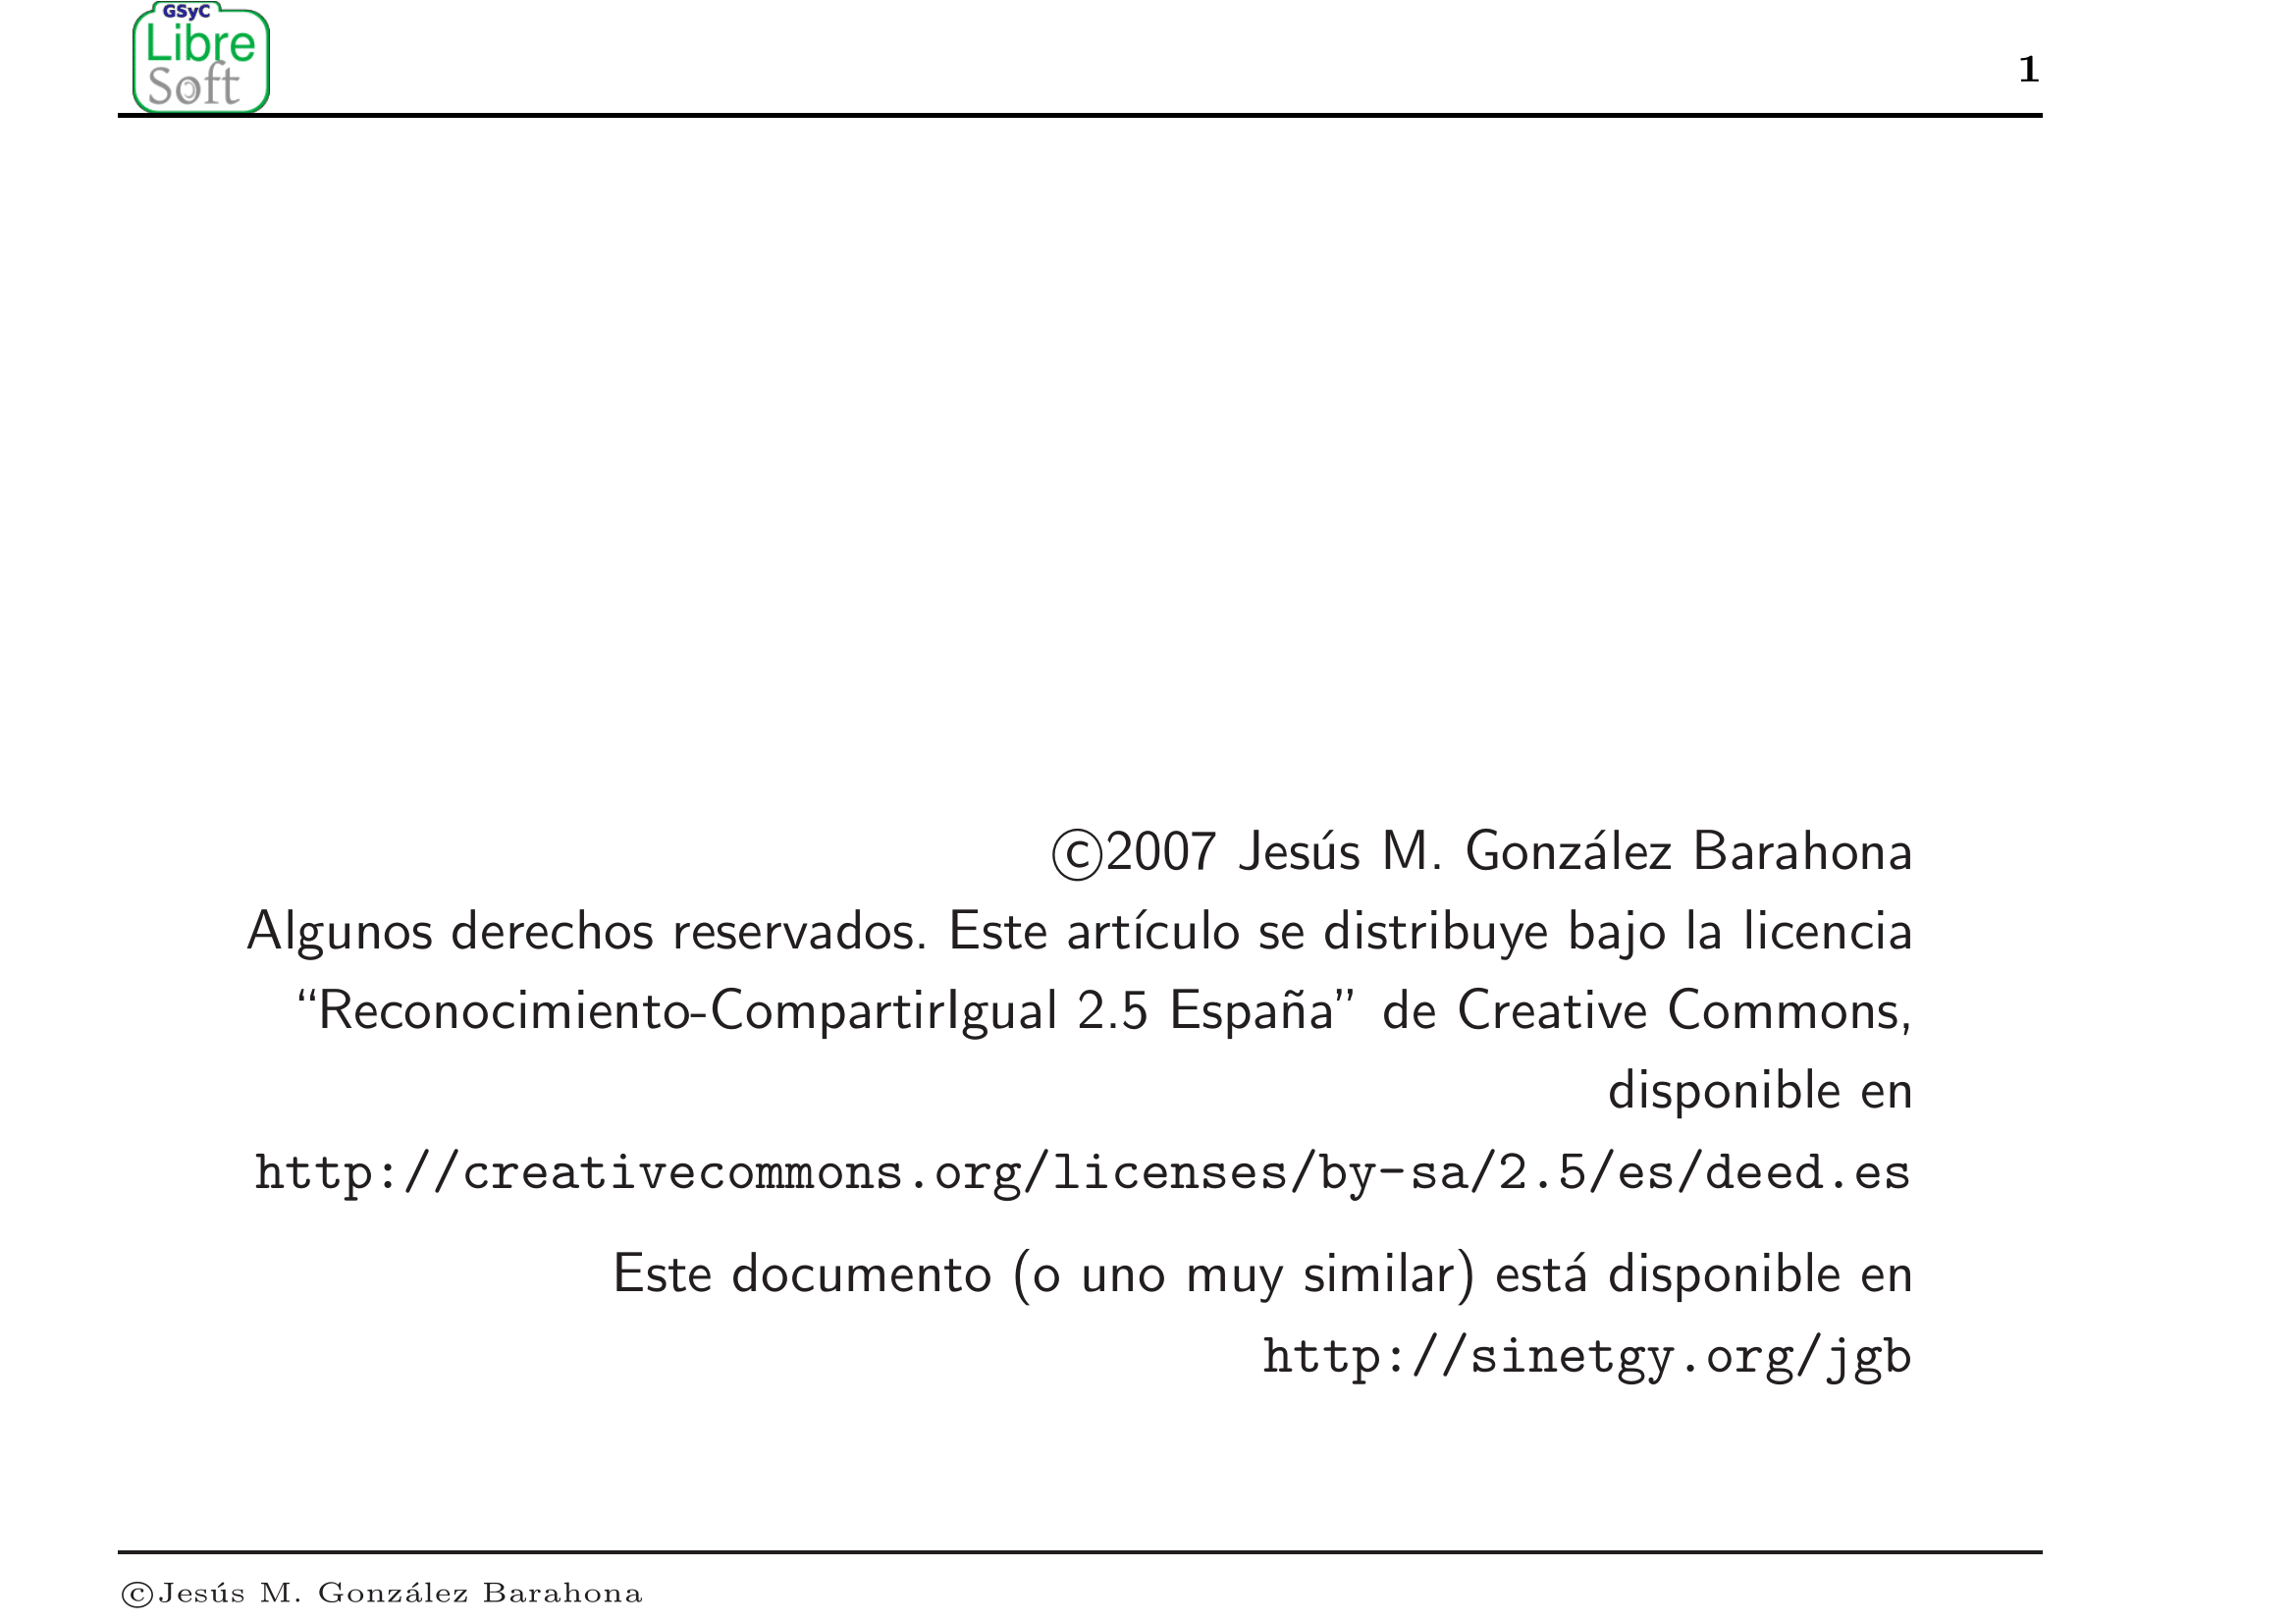
\includegraphics[width=12.5cm]{figs/transpas-02}
\end{center}  

\end{frame}

%%---------------------------------------------------------------
% LICENCIA DE REDISTRIBUCION DE LAS TRANSPAS
\frame{
~
\vspace{1.5cm}

\begin{flushright}
{\small
\copyright 2019 Jesús M. González Barahona. \\

  Algunos derechos reservados. \\
  Este documento se distribuye bajo la licencia \\
  ``Reconocimiento-CompartirIgual 3.0 España'' \\
  de Creative Commons, \\
  disponible en \\
}
{\footnotesize
  \url{https://creativecommons.org/licenses/by-sa/3.0/es/} \\
}

\vspace{.5cm}

{\small
Este documento está disponible en \\
\url{https://jgbarah.github.io/presentations} \\
}
\end{flushright}
}

\end{document}
